\documentclass{beamer}
% =============================================================================
% ENCODING
% =============================================================================
\usepackage[utf8]{inputenc}  % UTF-8 encoding support

% =============================================================================
% GRAPHICS
% =============================================================================
\usepackage{graphicx}  % For \includegraphics (401 uses across lectures)

% =============================================================================
% MATH PACKAGES
% =============================================================================
\usepackage{amsmath}    % For align, multline, equation environments (heavily used)
\usepackage{amsfonts}   % For \mathbb (e.g., \bbR, \bbE)
\usepackage{amssymb}    % For additional math symbols

% =============================================================================
% TABLES
% =============================================================================
\usepackage{booktabs}   % For \toprule, \midrule, \bottomrule (used in lecture13, lecture14)

% =============================================================================
% LISTS
% =============================================================================
\usepackage{enumerate}  % Enhanced enumerate environment (76 uses across lectures)

% =============================================================================
% TIKZ (DIAGRAMS)
% =============================================================================
\usepackage{tikz}       % For taxonomy diagram and footnotes positioning

% =============================================================================
% UTILITY PACKAGES
% =============================================================================
\usepackage{multido}    % For \multido command used in \eqpause
\usepackage{etoolbox}   % For \AtEndEnvironment, \ifbool, \newbool (used in preamble and taxonomy)
\usepackage{xspace}     % For smart spacing after custom commands (\ODESolve, \SDESolve)

% =============================================================================
% BEAMER THEME SETTINGS
% =============================================================================
\usetheme{default}
\usecolortheme{default}

\setbeamerfont{title}{size=\Huge}
\setbeamertemplate{footline}[frame number]{}
\setbeamertemplate{section in toc}[sections numbered]

\makeatletter
\newcommand\HUGE{\@setfontsize\Huge{35}{40}}
\makeatother    

\setbeamerfont{title}{size=\HUGE}
\beamertemplatenavigationsymbolsempty

% =============================================================================
% TIKZ LIBRARIES
% =============================================================================
% Used for taxonomy diagram: arrows, positioning, shapes
\usetikzlibrary{arrows.meta,calc,shapes,positioning,shadows,trees}

% =============================================================================
% CUSTOM FOOTNOTE COMMANDS
% =============================================================================
% \myfootnote{text} - creates a footnote at the bottom of the slide
\newcommand\myfootnote[1]{%
  \vspace{-0.5cm}%
  \tikz[remember picture,overlay]
  \draw (current page.south west) +(1in + \oddsidemargin,0.5em)
  node[anchor=south west,inner sep=0pt]{\parbox{\textwidth}{%
      \rlap{\rule{10em}{0.4pt}}\raggedright\scriptsize \textit{#1}}};}

% \myfootnotewithlink{url}{text} - creates a clickable footnote (623 uses across lectures)
\newcommand\myfootnotewithlink[2]{%
  \vspace{-0.5cm}%
  \tikz[remember picture,overlay]
  \draw (current page.south west) +(1in + \oddsidemargin,0.5em)
  node[anchor=south west,inner sep=0pt]{\parbox{\textwidth}{%
      \rlap{\rule{10em}{0.4pt}}\raggedright\scriptsize\href{#1}{\textit{#2}}}};}

% =============================================================================
% SECTION/SUBSECTION OUTLINE AUTOMATION
% =============================================================================
% Automatically show outline at the beginning of each section
\AtBeginSection[]
      {
      	\begin{frame}{Outline}
      		\tableofcontents[currentsection]
      	\end{frame}
      }
      \AtBeginSubsection[]{
      	\begin{frame}{Outline}
      		\tableofcontents[currentsection,currentsubsection]
      	\end{frame}
}

% =============================================================================
% CUSTOM SLIDE ANIMATION COMMANDS
% =============================================================================
% These commands enable step-by-step reveal of equations and content
% Used heavily across all lectures (1130+ uses of \nextonslide and \eqpause)

\newcounter{noscounter}   % Counter for \nextonslide (resets on each new slide)
\newcounter{pcounter}     % Counter for pause commands (resets after \eqpause)
\newcounter{diffcounter}  % Counts pauses after equations

% \nextonslide{content} - reveals content on the next overlay
\newcommand{\nextonslide}[1]{%
  \stepcounter{noscounter}%
  \stepcounter{pcounter}%
  \stepcounter{diffcounter}%
  \onslide<\value{noscounter}->{#1}%
}

% \resetonslide - resets all animation counters (called at each frame)
\newcommand{\resetonslide}{%
    \setcounter{noscounter}{1}%
    \setcounter{pcounter}{1}%
    \setcounter{diffcounter}{0}%
}

% \eqpause - pause after equation that syncs with \nextonslide
\newcommand{\eqpause}{%
  \multido{\i=1+1}{\value{pcounter}}{\pause}%
  \stepcounter{noscounter}%
  \setcounter{pcounter}{1}%
}

% \eqpausediff - helper command, runs automatically after math environments
\newcommand{\eqpausediff}{%
  \multido{\i=1+1}{\value{diffcounter}}{\pause}%
  \addtocounter{pcounter}{-\value{diffcounter}}%
  \setcounter{diffcounter}{0}%
}

% Apply \eqpausediff after math environments
\newcommand\AtEndBoth[2]{%
  \AtEndEnvironment{#1}{#2}%
  \AtEndEnvironment{#1*}{#2}%
}

\AtEndBoth{align}{\eqpausediff}
\AtEndBoth{equation}{\eqpausediff}
\AtEndBoth{multline}{\eqpausediff}

% Reset counters at the beginning of each frame
\addtobeamertemplate{frametitle}{\resetonslide}{}

% =============================================================================
% INCLUDE OTHER CONFIGURATION FILES
% =============================================================================
% ==============================================================================
% Custom LaTeX Commands for Deep Generative Models Course
% ==============================================================================

% ==============================================================================
% BOLD LETTERS (mathbf / boldsymbol)
% ==============================================================================

% ------------------------------------------------------------------------------
% Latin Bold Lowercase
% Usage: \bx for x in bold, commonly used for vectors
% ------------------------------------------------------------------------------
\newcommand{\ba}{\mathbf{a}}
\newcommand{\bc}{\mathbf{c}}
\newcommand{\be}{\mathbf{e}}
\newcommand{\bff}{\mathbf{f}}  % Note: \bf is reserved for bold font switching
\newcommand{\bg}{\mathbf{g}}
\newcommand{\bh}{\mathbf{h}}
\newcommand{\bp}{\mathbf{p}}
\newcommand{\bq}{\mathbf{q}}
\newcommand{\bs}{\mathbf{s}}
\newcommand{\bt}{\mathbf{t}}
\newcommand{\bu}{\mathbf{u}}
\newcommand{\bv}{\mathbf{v}}
\newcommand{\bw}{\mathbf{w}}
\newcommand{\bx}{\mathbf{x}}
\newcommand{\by}{\mathbf{y}}
\newcommand{\bz}{\mathbf{z}}
\newcommand{\bzero}{\boldsymbol{0}}  % Zero vector
\newcommand{\bone}{\mathbf{1}}       % Ones vector

% ------------------------------------------------------------------------------
% Latin Bold Uppercase
% Usage: \bX for X in bold, commonly used for matrices or random vectors
% ------------------------------------------------------------------------------
\newcommand{\bA}{\mathbf{A}}
\newcommand{\bG}{\mathbf{G}}
\newcommand{\bI}{\mathbf{I}}
\newcommand{\bJ}{\mathbf{J}}
\newcommand{\bL}{\mathbf{L}}
\newcommand{\bM}{\mathbf{M}}
\newcommand{\bP}{\mathbf{P}}
\newcommand{\bQ}{\mathbf{Q}}
\newcommand{\bR}{\mathbf{R}}
\newcommand{\bT}{\mathbf{T}}
\newcommand{\bU}{\mathbf{U}}
\newcommand{\bV}{\mathbf{V}}
\newcommand{\bW}{\mathbf{W}}
\newcommand{\bX}{\mathbf{X}}
\newcommand{\bZ}{\mathbf{Z}}

% ------------------------------------------------------------------------------
% Greek Bold Lowercase
% Usage: \btheta for θ in bold, commonly used for parameter vectors
% ------------------------------------------------------------------------------
\newcommand{\bepsilon}{\boldsymbol{\epsilon}}
\newcommand{\blambda}{\boldsymbol{\lambda}}
\newcommand{\bmu}{\boldsymbol{\mu}}
\newcommand{\bphi}{\boldsymbol{\phi}}
\newcommand{\bpi}{\boldsymbol{\pi}}
\newcommand{\bpsi}{\boldsymbol{\psi}}
\newcommand{\bsigma}{\boldsymbol{\sigma}}
\newcommand{\btheta}{\boldsymbol{\theta}}

% ------------------------------------------------------------------------------
% Greek Bold Uppercase
% Usage: \bSigma for Σ in bold, commonly used for covariance matrices
% ------------------------------------------------------------------------------
\newcommand{\bPhi}{\boldsymbol{\Phi}}
\newcommand{\bSigma}{\boldsymbol{\Sigma}}
\newcommand{\bTheta}{\boldsymbol{\Theta}}

% ==============================================================================
% CALLIGRAPHIC LETTERS (mathcal)
% Usage: \cX for calligraphic X, commonly used for sets and spaces
% ==============================================================================
\newcommand{\cF}{\mathcal{F}}
\newcommand{\cI}{\mathcal{I}}
\newcommand{\cL}{\mathcal{L}}
\newcommand{\cM}{\mathcal{M}}
\newcommand{\cN}{\mathcal{N}}
\newcommand{\cO}{\mathcal{O}}
\newcommand{\cP}{\mathcal{P}}
\newcommand{\cS}{\mathcal{S}}
\newcommand{\cT}{\mathcal{T}}
\newcommand{\cW}{\mathcal{W}}
\newcommand{\cX}{\mathcal{X}}
\newcommand{\cZ}{\mathcal{Z}}

% ==============================================================================
% BLACKBOARD BOLD LETTERS (mathbb)
% Usage: \bbR for ℝ, commonly used for number sets and expectations
% ==============================================================================
\newcommand{\bbE}{\mathbb{E}}  % Expectation
\newcommand{\bbI}{\mathbb{I}}  % Indicator function
\newcommand{\bbP}{\mathbb{P}}  % Probability measure
\newcommand{\bbR}{\mathbb{R}}  % Real numbers

% ==============================================================================
% MATH OPERATORS
% ==============================================================================

% ------------------------------------------------------------------------------
% Optimization Operators
% Usage: \argmin_{x} f(x) for proper spacing and limits placement
% ------------------------------------------------------------------------------
\DeclareMathOperator*{\argmin}{arg\,min}
\DeclareMathOperator*{\argmax}{arg\,max}

% ------------------------------------------------------------------------------
% Statistical Operators
% Usage: \cov(X, Y) for covariance
% ------------------------------------------------------------------------------
\DeclareMathOperator{\cov}{cov}

% ------------------------------------------------------------------------------
% Linear Algebra Operators
% Usage: \tr(\bA) for trace of matrix A
% ------------------------------------------------------------------------------
\DeclareMathOperator{\tr}{tr}

% ------------------------------------------------------------------------------
% Other Mathematical Operators
% ------------------------------------------------------------------------------
\DeclareMathOperator{\diver}{div}      % Divergence (vector calculus)
\newcommand{\sg}{\mathrm{sg}}          % Stop-gradient operator
\DeclareMathOperator{\softmax}{softmax}
\DeclareMathOperator{\supp}{supp}      % Support of a distribution

% ==============================================================================
% PROBABILITY DISTRIBUTIONS
% Usage: X \sim \cN(0, 1), Y \sim \Bern(p)
% ==============================================================================
\DeclareMathOperator{\Bern}{Bern}      % Bernoulli distribution
\DeclareMathOperator{\Cat}{Cat}        % Categorical distribution
\DeclareMathOperator{\Gumbel}{Gumbel}  % Gumbel distribution
\DeclareMathOperator{\Uniform}{Uniform}

% ==============================================================================
% METRICS AND DIVERGENCES
% Usage: \KL(p \| q), \JSD(p, q)
% ==============================================================================
\newcommand{\Ent}{\mathrm{H}}          % Entropy
\newcommand{\FID}{\mathrm{FID}}        % Fréchet Inception Distance
\newcommand{\JSD}{D_\mathrm{JS}}        % Jensen-Shannon Divergence
\newcommand{\KL}{D_\mathrm{KL}}        % Kullback-Leibler Divergence
\DeclareMathOperator{\MMD}{MMD}        % Maximum Mean Discrepancy
\DeclareMathOperator{\SNR}{SNR}        % Signal-to-Noise Ratio

% ==============================================================================
% NEURAL NETWORK NOTATION
% ==============================================================================

% ------------------------------------------------------------------------------
% Network Architectures (upright font for abbreviations)
% Usage: f_{\btheta} = \NN_{\btheta}(\bx)
% ------------------------------------------------------------------------------
\newcommand{\MLP}{\mathrm{MLP}}        % Multi-Layer Perceptron
\newcommand{\NN}{\mathrm{NN}}          % Neural Network
\newcommand{\RNN}{\mathrm{RNN}}        % Recurrent Neural Network

% ------------------------------------------------------------------------------
% Numerical Solvers (monospace font)
% Usage: \bx_T = \ODESolve(v, \bx_0, T)
% ------------------------------------------------------------------------------
\newcommand{\ODESolve}{\texttt{ODESolve}\xspace}
\newcommand{\SDESolve}{\texttt{SDESolve}\xspace}

% ==============================================================================
% COMMON SHORTCUTS
% Usage: Frequently used subscripted or parameterized expressions
% ==============================================================================
\newcommand{\pd}{p_{\text{data}}}              % Data distribution
\newcommand{\pt}{p_{\boldsymbol{\theta}}}      % Parameterized distribution
\newcommand{\qagg}{q_{\text{agg}}}             % Aggregated posterior
\newcommand{\lambdamax}{\lambda_{\text{max}}}  % Maximum eigenvalue
  % Math shorthand commands (\bx, \bbE, \KL, etc.)
\input{../utils/title}        % Title page template
% For each possible node, we create a boolean
\newbool{hl@root}
\newbool{hl@explicit}
\newbool{hl@implicit}
\newbool{hl@exact}
\newbool{hl@approx}
\newbool{hl@gan}
\newbool{hl@ar}
\newbool{hl@nf}
\newbool{hl@vae}
\newbool{hl@score}
\newbool{hl@cont}
\newbool{hl@ddpm}
\newbool{hl@sm}
\newbool{hl@ode}
\newbool{hl@sde}
\newbool{hl@fm}

% Command to reset all bools
\newcommand{\resetAllHighlights}{%
    \boolfalse{hl@root}%
    \boolfalse{hl@explicit}%
    \boolfalse{hl@implicit}%
    \boolfalse{hl@exact}%
    \boolfalse{hl@approx}%
    \boolfalse{hl@gan}%
    \boolfalse{hl@ar}%
    \boolfalse{hl@nf}%
    \boolfalse{hl@vae}%
    \boolfalse{hl@score}%
    \boolfalse{hl@cont}%
    \boolfalse{hl@ddpm}%
    \boolfalse{hl@sm}%
    \boolfalse{hl@ode}%
    \boolfalse{hl@sde}%
    \boolfalse{hl@fm}%
}

% Command to set a single highlight
\newcommand{\setHighlight}[1]{%
    \booltrue{hl@#1}%
}

% Command to set highlights from comma-separated list
\newcommand{\setHighlights}[1]{%
    \resetAllHighlights%
    \forcsvlist{\setHighlight}{#1}%
}

% Highlighted style definition
\tikzset{
    hl/.style={line width=1.2pt, draw=black, font=\scriptsize\bfseries},
    box/.style={
        rectangle, 
        draw=gray!50, 
        rounded corners=2pt, 
        minimum width=1.9cm, 
        minimum height=0.5cm, 
        align=center, 
        font=\scriptsize, 
        line width=0.4pt
    },
    rootnode/.style={box, fill=violet!20},
    category/.style={box, fill=teal!20},
    model/.style={box, fill=yellow!30},
    arrow/.style={-Stealth, draw=gray!80, line width=0.4pt}
}

% Draw taxonomy with pre-set highlights
\newcommand{\drawTaxonomy}{%
    \begin{tikzpicture}[scale=0.9, transform shape, node distance=0.6cm and 0.3cm]
        % --- CENTRAL ROOT ---
        \ifbool{hl@root}{\node[rootnode, hl] (root) {Generative Models};}{\node[rootnode] (root) {Generative Models};}

        % --- UPPER BRANCHES ---
        \ifbool{hl@explicit}{\node[category, hl, above left=0.6cm and 0.5cm of root] (explicit) {Explicit density};}{\node[category, above left=0.6cm and 0.5cm of root] (explicit) {Explicit density};}
        \ifbool{hl@implicit}{\node[category, hl, above right=0.6cm and 0.5cm of root] (implicit) {Implicit density};}{\node[category, above right=0.6cm and 0.5cm of root] (implicit) {Implicit density};}

        \ifbool{hl@exact}{\node[category, hl, above left=0.6cm and -0.6cm of explicit] (exact) {Exact likelihood};}{\node[category, above left=0.6cm and -0.6cm of explicit] (exact) {Exact likelihood};}
        \ifbool{hl@approx}{\node[category, hl, above right=0.6cm and -0.6cm of explicit] (approx) {Approximate likelihood};}{\node[category, above right=0.6cm and -0.6cm of explicit] (approx) {Approximate likelihood};}

        \ifbool{hl@gan}{\node[model, hl, above=0.6cm of implicit] (gans) {GANs};}{\node[model, above=0.6cm of implicit] (gans) {GANs};}

        \ifbool{hl@ar}{\node[model, hl, above left=0.6cm and -0.9cm of exact] (ar) {Autoregressive \\ models};}{\node[model, above left=0.6cm and -0.9cm of exact] (ar) {Autoregressive \\ models};}
        \ifbool{hl@nf}{\node[model, hl, above right=0.6cm and -0.9cm of exact] (nf) {Normalizing \\ Flows};}{\node[model, above right=0.6cm and -0.9cm of exact] (nf) {Normalizing \\ Flows};}
        \ifbool{hl@vae}{\node[model, hl, above=0.6cm of approx] (vae) {Variational \\ Autoencoders};}{\node[model, above=0.6cm of approx] (vae) {Variational \\ Autoencoders};}

        % --- LOWER BRANCHES ---
        \ifbool{hl@score}{\node[category, hl, below left=0.6cm and 0.5cm of root] (score) {Score-based};}{\node[category, below left=0.6cm and 0.5cm of root] (score) {Score-based};}
        \ifbool{hl@cont}{\node[category, hl, below right=0.6cm and 0.5cm of root] (cont) {Continuous \\ dynamics};}{\node[category, below right=0.6cm and 0.5cm of root] (cont) {Continuous \\ dynamics};}

        \ifbool{hl@sm}{\node[model, hl, below left=0.6cm and -0.8cm of score] (sm) {Score Matching};}{\node[model, below left=0.6cm and -0.8cm of score] (sm) {Score Matching};}
        \ifbool{hl@ddpm}{\node[model, hl, below right=0.6cm and -0.8cm of score] (ddpm) {Denoising Diffusion};}{\node[model, below right=0.6cm and -0.8cm of score] (ddpm) {Denoising Diffusion};}

        \ifbool{hl@ode}{\node[model, hl, below left=0.6cm and -0.8cm of cont] (ode) {Neural ODEs};}{\node[model, below left=0.6cm and -0.8cm of cont] (ode) {Neural ODEs};}
        \ifbool{hl@sde}{\node[model, hl, below right=0.6cm and -0.8cm of cont] (sde) {SDE-based \\ Diffusion};}{\node[model, below right=0.6cm and -0.8cm of cont] (sde) {SDE-based \\ Diffusion};}

        \ifbool{hl@fm}{\node[model, hl, below=0.6cm of ode] (fm) {Flow Matching};}{\node[model, below=0.6cm of ode] (fm) {Flow Matching};}

        % --- CONNECTIONS ---
        \draw[arrow] (root.north) -- ++(0,0.3) -| (explicit.south);
        \draw[arrow] (root.north) -- ++(0,0.3) -| (implicit.south);
        \draw[arrow] (root.south) -- ++(0,-0.3) -| (score.north);
        \draw[arrow] (root.south) -- ++(0,-0.3) -| (cont.north);
        \draw[arrow] (explicit.north) -- ++(0,0.3) -| (exact.south);
        \draw[arrow] (explicit.north) -- ++(0,0.3) -| (approx.south);
        \draw[arrow] (exact.north) -- ++(0,0.3) -| (ar.south);
        \draw[arrow] (exact.north) -- ++(0,0.3) -| (nf.south);
        \draw[arrow] (approx.north) -- (vae.south);
        \draw[arrow] (implicit.north) -- (gans.south);
        \draw[arrow] (score.south) -- ++(0,-0.3) -| (sm.north);
        \draw[arrow] (score.south) -- ++(0,-0.3) -| (ddpm.north);
        \draw[arrow] (cont.south) -- ++(0,-0.3) -| (ode.north);
        \draw[arrow] (cont.south) -- ++(0,-0.3) -| (sde.north);
        \draw[arrow] (ode.south) -- (fm.north);
    \end{tikzpicture}
}

% The main taxonomy rendering command
\newcommand{\renderTaxonomy}[1]{%
    \setHighlights{#1}%
    \centering
    \drawTaxonomy%
}     % Generative models taxonomy diagram

\createdgmtitle{8}
%--------------------------------------------------------------------------------
\begin{document}
%--------------------------------------------------------------------------------
\begin{frame}[noframenumbering,plain]
\titlepage
\end{frame}
%=======
\begin{frame}{Recap of Previous Lecture}
    \myfootnotewithlink{https://arxiv.org/abs/2403.18103}{Chan S. Tutorial on Diffusion Models for Imaging and Vision, 2024}
    \begin{block}{Forward Gaussian Diffusion Process}
        Let $\bx_0 = \bx \sim \pd(\bx)$, $\beta_t \ll 1$, $\alpha_t = 1 - \beta_t$ and $\bar{\alpha}_t = \prod_{s=1}^t \alpha_s$. 
        \begin{align*}
            \bx_t &= \sqrt{1 - \beta_t} \cdot \bx_{t - 1} + \sqrt{\beta_t} \cdot \bepsilon, \quad \text{where }\bepsilon \sim \cN(0, \bI); \\
            \bx_t &= \sqrt{\bar{\alpha}_t} \cdot \bx_{0} + \sqrt{1 - \bar{\alpha}_t} \cdot \bepsilon, \quad \text{where } \bepsilon \sim \cN(0, \bI).
        \end{align*}
        \vspace{-0.6cm}
        \begin{align*}
            q(\bx_t | \bx_{t-1}) &= \cN(\sqrt{1 - \beta_t} \cdot \bx_{t-1}, \beta_t \cdot \bI); \\
            q(\bx_t | \bx_0) &= \cN(\sqrt{\bar{\alpha}_t} \cdot \bx_0, (1 - \bar{\alpha}_t) \cdot \bI).
        \end{align*}
        \vspace{-0.6cm}
    \end{block}
    \begin{figure}
        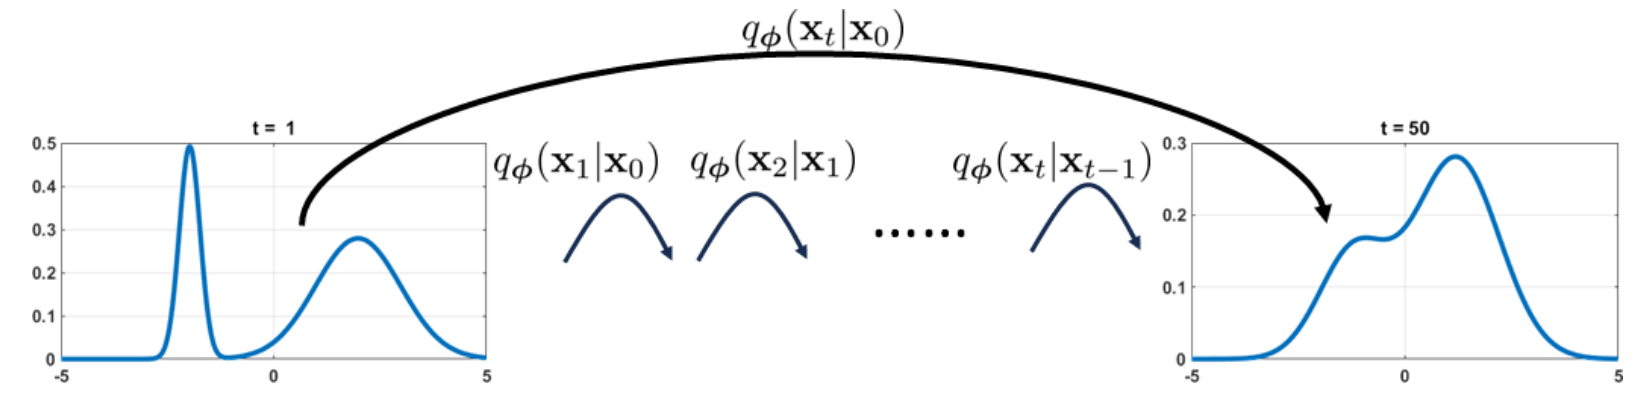
\includegraphics[width=0.8\linewidth]{figs/conditional_diffusion}
    \end{figure}
\end{frame}
%=======
\begin{frame}{Recap of Previous Lecture}
    \myfootnotewithlink{https://ayandas.me/blog-tut/2021/12/04/diffusion-prob-models.html}{Das A. An Introduction to Diffusion Probabilistic Models, blog post, 2021}
    \textbf{Diffusion} describes the process where particles migrate from regions of high density to regions of low density.
    \vspace{-0.2cm}
    \begin{figure}
        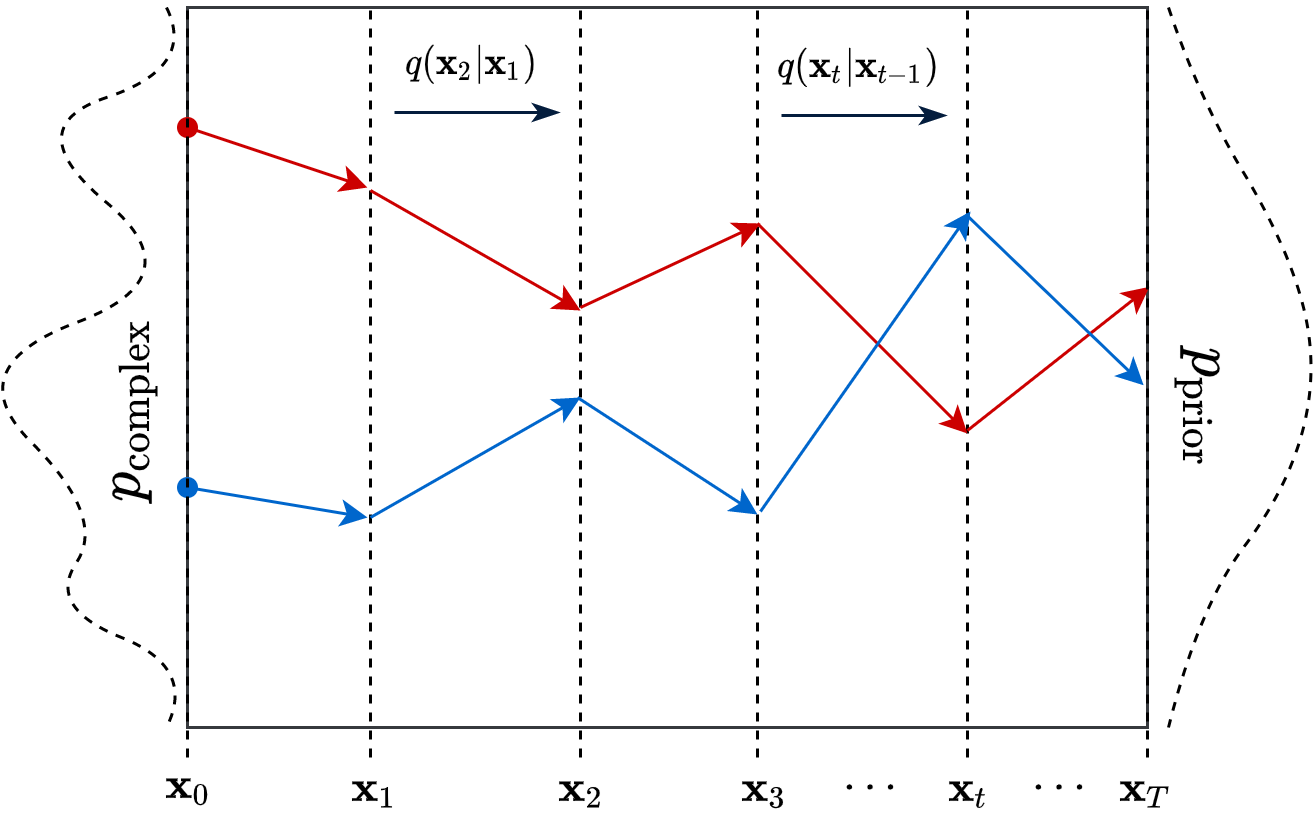
\includegraphics[width=0.5\linewidth]{figs/diffusion_over_time}
    \end{figure}
    \vspace{-0.6cm}
    \begin{enumerate}
        \item $\bx_0 = \bx \sim \pd(\bx)$;
        \item $\bx_t = \sqrt{1 - \beta_t} \cdot \bx_{t - 1} + \sqrt{\beta_t} \cdot \bepsilon$, with $\bepsilon \sim \cN(0, \bI)$, $t \geq 1$;
        \item $\bx_T \sim p_{\infty}(\bx) = \cN(0, \bI)$, for $T \gg 1$.
    \end{enumerate}
    If we can invert this process, we would have a way to sample $\bx \sim \pd(\bx)$ using noise samples, i.e. $p_{\infty}(\bx) = \cN(0, \bI)$. \\ 
    Hence, our objective becomes to reverse this process.
\end{frame}
%=======
\begin{frame}{Recap of Previous Lecture}
    \myfootnotewithlink{https://lilianweng.github.io/posts/2021-07-11-diffusion-models/}{Weng L. What are Diffusion Models?, blog post, 2021}
    \vspace{-0.3cm}
    \begin{figure}
        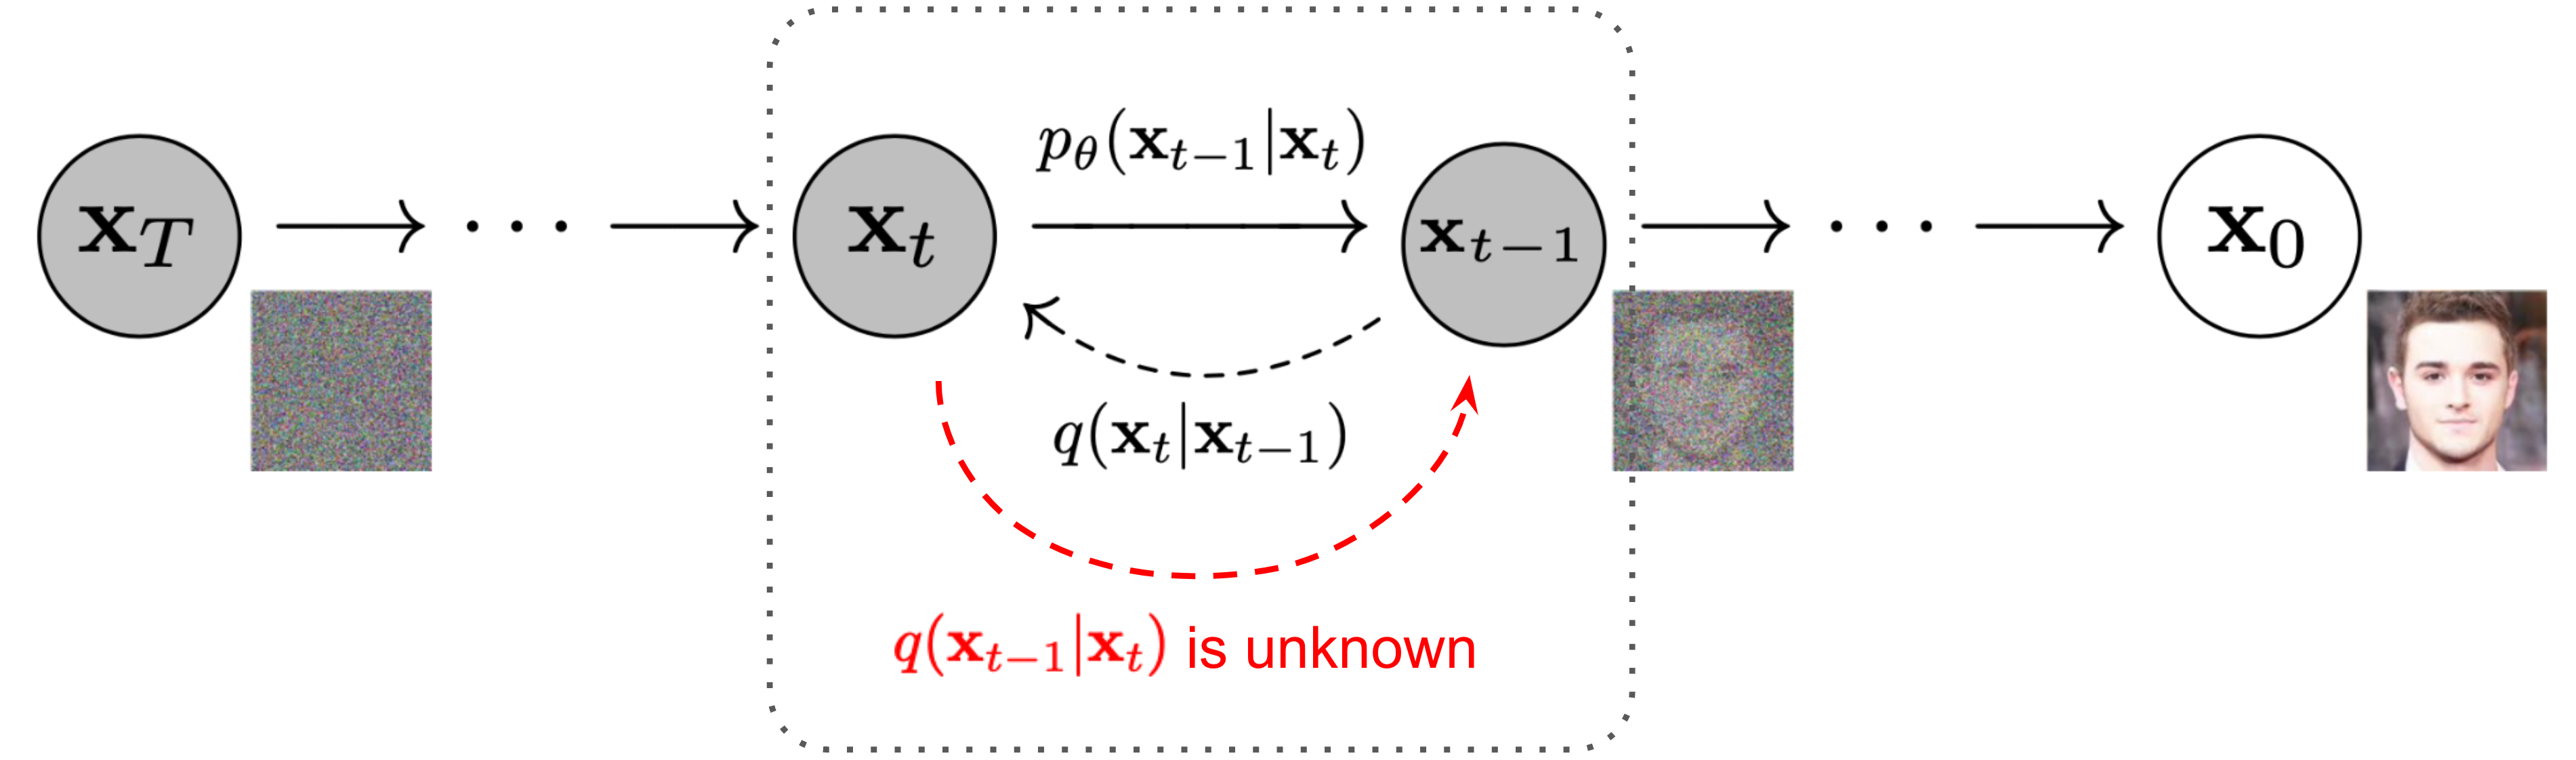
\includegraphics[width=0.8\linewidth]{figs/DDPM}
    \end{figure}
    \vspace{-0.5cm}
    \begin{block}{Reverse Process (Ancestral Sampling)}
        \vspace{-0.5cm}
        {\small
        \[
            q(\bx_{t-1}|\bx_{t}) = \frac{q(\bx_{t}|\bx_{t-1}) {\color{violet}q(\bx_{t-1})}}{{\color{violet}q(\bx_{t})}} \approx \pt(\bx_{t - 1} | \bx_t) = \cN \left(\bmu_{\btheta, t}(\bx_t), \bsigma_{\btheta, t}^2(\bx_t)\right)
        \]}
        {\color{gray}The Feller theorem guarantees this approximation is valid.}
    \end{block}
    \begin{minipage}{0.5\linewidth}
        \begin{block}{Forward Process}
            \begin{enumerate}
                \item $\bx_0 = \bx \sim \pd(\bx)$;
                \item $\bx_t = \sqrt{1 - \beta_t} \cdot \bx_{t - 1} + \sqrt{\beta_t} \cdot \bepsilon$;
                \item $\bx_T \sim p_{\infty}(\bx) = \cN(0, \bI)$.
            \end{enumerate}
        \end{block}
    \end{minipage}%
    \begin{minipage}{0.55\linewidth}
        \begin{block}{Reverse Process}
            \begin{enumerate}
                \item $\bx_T \sim p_{\infty}(\bx) = \cN(0, \bI)$;
                \item $\bx_{t - 1} = \bsigma_{\btheta, t}(\bx_t) \cdot \bepsilon + \bmu_{\btheta, t}(\bx_t)$;
                \item $\bx_0 = \bx \sim \pd(\bx)$;
            \end{enumerate}
        \end{block}
    \end{minipage}
\end{frame}
%=======
\begin{frame}{Recap of Previous Lecture}
	\myfootnotewithlink{https://arxiv.org/abs/2006.11239}{Ho J. Denoising Diffusion Probabilistic Models, 2020}

	\textbf{Forward Process}: Converts an arbitrary distribution $\pd(\bx)$ into the standard normal $\cN(0, \bI)$ by incrementally adding noise.
	\begin{align*}
		q(\bx_t | \bx_{t-1}) &= \cN(\sqrt{1 - \beta_t}\, \bx_{t-1}, \beta_t\, \bI); \\
		q(\bx_t | \bx_0) &= \cN(\sqrt{\bar{\alpha}_t}\, \bx_0, (1 - \bar{\alpha}_t)\, \bI).
	\end{align*}
	\textbf{Reverse Process}: This intractable distribution can be well-approximated by a Gaussian (with unknown parameters) when $\beta_t$ is sufficiently small.
	\[
		q(\bx_{t-1}|\bx_{t}) = \frac{q(\bx_{t}|\bx_{t-1}) q(\bx_{t-1})}{q(\bx_{t})} \approx \cN \left(\bmu_{\btheta, t}(\bx_t), \bsigma_{\btheta, t}^2(\bx_t)\right)
	\]
	\textbf{Conditioned Reverse Process}: This Gaussian, with known parameters, describes how to denoise a noisy image~$\bx_t$ when the final clean image~$\bx_0$ is known.
	\vspace{-0.3cm}
	\[
		q(\bx_{t-1}|\bx_{t}, {\color{olive}\bx_0}) = \cN(\tilde{\bmu}_t(\bx_t, \bx_0), \tilde{\beta}_t\, \bI)
	\]
\end{frame}
%=======
\begin{frame}{Recap of Previous Lecture}
	\myfootnotewithlink{https://ayandas.me/blog-tut/2021/12/04/diffusion-prob-models.html}{Das A. An introduction to Diffusion Probabilistic Models, blog post, 2021}
	\begin{itemize}
		\item $\bz = (\bx_1, \dots, \bx_T)$ represents the latent variables.
		\item Variational posterior distribution:
		\vspace{-0.2cm}
		\[
			q(\bz | \bx) = q(\bx_1, \dots, \bx_T | \bx_0) = \prod_{t = 1}^T q(\bx_t | \bx_{t - 1}).
		\]
		\vspace{-0.3cm}
		\item Generative model and prior:
		\vspace{-0.2cm}
		\[
			\pt(\bx | \bz) = \pt(\bx_0 | \bx_1); \quad 
			\pt(\bz) = \prod_{t=2}^\top \pt(\bx_{t - 1} | \bx_t) \cdot p(\bx_T)
		\]
	\end{itemize}
	\vspace{-0.2cm}
	\begin{block}{ELBO}
		\vspace{-0.2cm}
		\[
			\log \pt(\bx) \geq \bbE_{q({\color{teal}\bz} | \bx)} \log \frac{\pt(\bx, {\color{teal}\bz})}{q({\color{teal}\bz} | \bx)} = \cL_{\bphi, \btheta}(\bx) \rightarrow \max_{q, \btheta}
		\]
		\vspace{-0.5cm}
		\begin{multline*}
			\cL_{\bphi, \btheta}(\bx) =  {\color{olive}\bbE_{q(\bx_1 | \bx_0)} \log \pt(\bx_0 | \bx_1)} - {\color{violet}\KL\bigl(q(\bx_T | \bx_0) \| p(\bx_T)\bigr)} - \\
			- \sum_{t=2}^\top  \underbrace{ \bbE_{q(\bx_t | \bx_0)}\KL \bigl(q(\bx_{t-1} | \bx_t, \bx_0) \| \pt(\bx_{t-1} | \bx_t)\bigr)}_{\cL_t}
		\end{multline*}
	\end{block}
\end{frame}
%=======
\begin{frame}{Outline}
    \tableofcontents
\end{frame}
%=======
\section{Diffusion ELBO Derivation (continued)}
%=======
\begin{frame}{ELBO for Gaussian Diffusion Model}
    \myfootnotewithlink{https://arxiv.org/abs/2208.11970}{Luo C. Understanding Diffusion Models: A Unified Perspective, 2022}
    \begin{figure}
        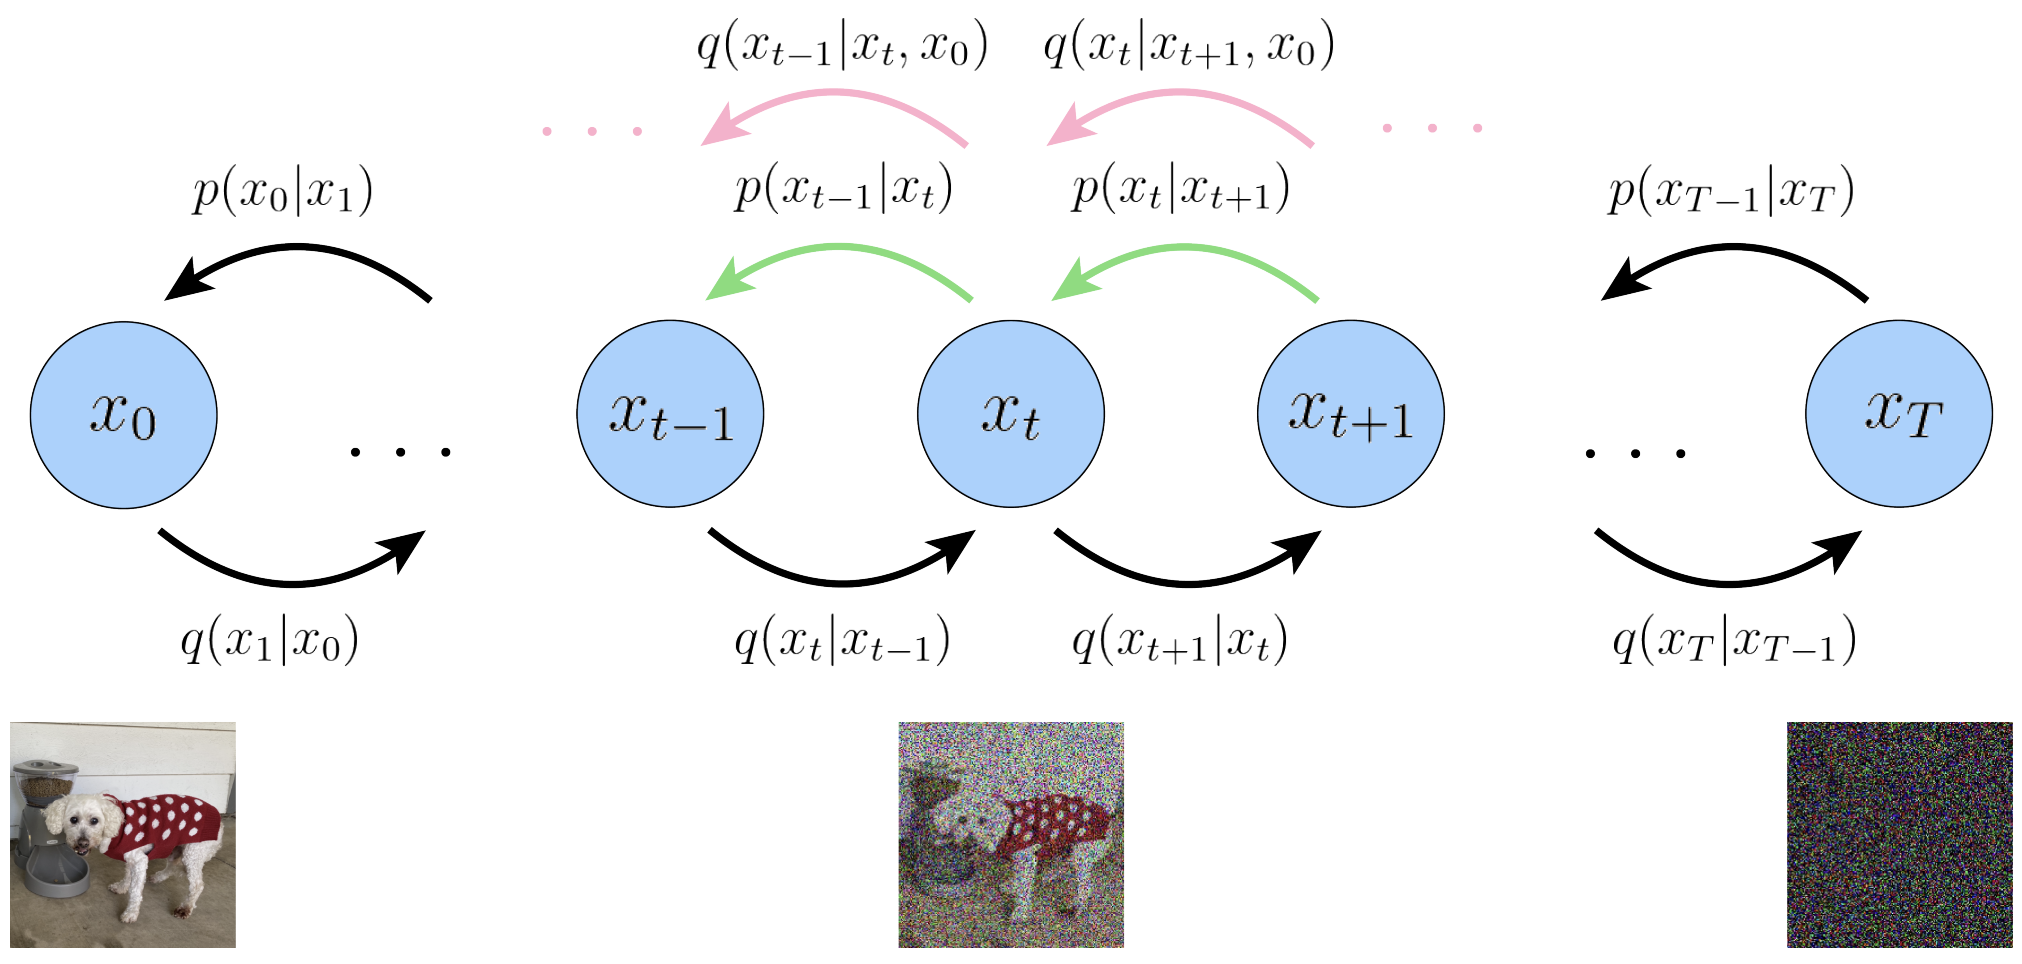
\includegraphics[width=\linewidth]{figs/diffusion_objective}
    \end{figure}
    \[
        \cL_t = \bbE_{q(\bx_t | \bx_0)} \KL \bigl(q(\bx_{t-1} | \bx_t, \bx_0) \| \pt(\bx_{t-1} | \bx_t)\bigr)
    \]
    \begin{align*}
        q(\bx_{t-1} | \bx_t, \bx_0) &= \cN(\bx_{t-1} | \tilde{\bmu}_t(\bx_t, \bx_0), \tilde{\beta}_t \bI), \\
        \pt(\bx_{t - 1} | \bx_t) &= \cN \bigl(\bx_{t - 1} | \bmu_{\btheta, t}(\bx_t), \bsigma_{\btheta, t}^2(\bx_t)\bigr)
    \end{align*}
\end{frame}
%=======
\begin{frame}{ELBO for Gaussian Diffusion Model}
    \myfootnotewithlink{https://arxiv.org/abs/2006.11239}{Ho J. Denoising Diffusion Probabilistic Models, 2020}
    \[
        \cL_t = \bbE_{q(\bx_t | \bx_0)} \KL \bigl(q(\bx_{t-1} | \bx_t, \bx_0) \| \pt(\bx_{t-1} | \bx_t)\bigr)
    \]
    \vspace{-0.7cm}
    \begin{align*}
        q(\bx_{t-1} | \bx_t, \bx_0) &= \cN(\bx_{t-1} | \tilde{\bmu}_t(\bx_t, \bx_0), \tilde{\beta}_t \bI), \\
        \pt(\bx_{t - 1} | \bx_t) &= \cN \bigl(\bx_{t - 1} | \bmu_{\btheta, t}(\bx_t), {\color{violet}\bsigma_{\btheta, t}^2(\bx_t)}\bigr)
    \end{align*}
    \eqpause
    Let's assume that
    \[
        {\color{violet}\bsigma_{\btheta, t}^2(\bx_t) = \tilde{\beta}_t \bI} \quad \Rightarrow \quad \pt(\bx_{t - 1} | \bx_t) = \cN \bigl(\bx_{t - 1} | \bmu_{\btheta, t}(\bx_t), {\color{violet}\tilde{\beta}_t \bI} \bigr).
    \]
    \eqpause
    Theoretically, the optimal $\bsigma_{\btheta, t}^2(\bx_t)$ lies in $[\tilde{\beta}_t, \beta_t]$:
    \begin{itemize}
        \item $\beta_t$ is optimal for $\bx_0 \sim \cN(0, \bI)$;
        \item $\tilde{\beta}_t$ is optimal for $\bx_0 \sim \delta(\bx_0 - \bx^*)$.
    \end{itemize}
    \eqpause
    \begin{align*}
        \cL_t &= \bbE_{q(\bx_t | \bx_0)} KL\Bigl(\cN\bigl(\tilde{\bmu}_t(\bx_t, \bx_0), \tilde{\beta}_t \bI \bigr) \| \cN\bigl(\bmu_{\btheta, t}(\bx_t), \tilde{\beta}_t \bI\bigr)\Bigr) \\ 
        \nextonslide{&= \bbE_{q(\bx_t | \bx_0)} \left[\frac{1}{2\tilde{\beta}_t} \bigl\| \tilde{\bmu}_t(\bx_t, \bx_0) - \bmu_{\btheta, t}(\bx_t) \bigr\|^2  \right]}
    \end{align*}
\end{frame}
%=======
\begin{frame}{ELBO for Gaussian Diffusion Model}
    \myfootnotewithlink{https://arxiv.org/abs/2006.11239}{Ho J. Denoising Diffusion Probabilistic Models, 2020}
    \begin{block}{Training}
        \begin{enumerate}
            \item Obtain a sample $\bx_0 \sim \pd(\bx)$.
            \item Generate a noisy image $\bx_t = \sqrt{\bar{\alpha}_t} \cdot \bx_0 + \sqrt{1 - \bar{\alpha}_t} \cdot \bepsilon$, with $\bepsilon \sim \cN(0, \bI)$.
            \item Compute the ELBO
            \vspace{-0.3cm}
            \begin{multline*}
                \cL_{\bphi, \btheta}(\bx) =  {\color{olive}\bbE_{q(\bx_1 | \bx_0)} \log \pt(\bx_0 | \bx_1)} - {\color{violet}\KL\bigl(q(\bx_T | \bx_0) \| p(\bx_T)\bigr)} - \\
                - {\color{teal}\sum_{t=2}^T \underbrace{ \bbE_{q(\bx_t | \bx_0)} \left[\frac{1}{2\tilde{\beta}_t} \bigl\| \tilde{\bmu}_t(\bx_t, \bx_0) - \bmu_{\btheta, t}(\bx_t) \bigr\|^2  \right]}_{\cL_t}}
            \end{multline*}
            \vspace{-0.7cm}
        \end{enumerate}
    \end{block}
    \eqpause
    \begin{block}{Sampling}
        \begin{enumerate}
            \item Sample $\bx_T \sim \cN(0, \bI)$.
            \item Denoise: $\bx_{t - 1} = \bmu_{\btheta, t}(\bx_t) +  \sqrt{\tilde{\beta}_t} \cdot \bepsilon$, $\bepsilon \sim \cN(0, \bI)$.
        \end{enumerate}
    \end{block}
\end{frame}
%=======
\section{Gaussian Diffusion Reparametrization}
%=======
\begin{frame}{Reparametrization of DDPM}
    \myfootnotewithlink{https://arxiv.org/abs/2006.11239}{Ho J. Denoising Diffusion Probabilistic Models, 2020}
    \[
        \cL_t = \bbE_{q(\bx_t | \bx_0)} \left[\frac{1}{2\tilde{\beta}_t} \bigl\| \tilde{\bmu}_t(\bx_t, \bx_0) - \bmu_{\btheta, t}(\bx_t) \bigr\|^2  \right]
    \]
    \[
        \tilde{\bmu}_t(\bx_t, \bx_0) = \frac{\sqrt{\alpha_t}(1 - \bar{\alpha}_{t-1})}{1 - \bar{\alpha}_t} \cdot \bx_t + \frac{\sqrt{\bar{\alpha}_{t-1}}(1 - \alpha_t)}{1 - \bar{\alpha}_t} \cdot {\color{olive} \bx_0}
    \]
    \eqpause
    \vspace{-0.2cm}
    \[
        \bx_t = \sqrt{\bar{\alpha}_t} \cdot \bx_0 + \sqrt{1 - \bar{\alpha}_t} \cdot \bepsilon \quad \nextonslide{\Rightarrow \quad {\color{olive} \bx_0} = \frac{\bx_t -  \sqrt{1 - \bar{\alpha}_t} \cdot \bepsilon}{\sqrt{\bar{\alpha}_t}}}
    \]
    \eqpause
    \vspace{-0.3cm}
    \begin{itemize}
        \item There is a linear relationship between $\bepsilon$, $\bx_t$, and $\bx_0$.
        \item Let's try to rewrite this mean using only $\bx_t$ and $\bepsilon$.
    \end{itemize}
    \eqpause
    \vspace{-0.2cm}
    \begin{align*}
        \tilde{\bmu}_t(\bx_t, \bepsilon) &= \frac{\sqrt{\alpha_t}(1 - \bar{\alpha}_{t-1})}{1 - \bar{\alpha}_t} \cdot \bx_t + \frac{\sqrt{\bar{\alpha}_{t-1}}(1 - \alpha_t)}{1 - \bar{\alpha}_t} \cdot {\color{olive} \left(\frac{\bx_t -  \sqrt{1 - \bar{\alpha}_t} \cdot \bepsilon}{\sqrt{\bar{\alpha}_t}}\right)} \\
        \nextonslide{&= \frac{1}{\sqrt{\alpha_t}} \cdot \bx_t - \frac{1 - \alpha_t}{\sqrt{\alpha_t (1 - \bar{\alpha}_t)}} \cdot \bepsilon}
    \end{align*}
\end{frame}
%=======
\begin{frame}{Reparametrization of DDPM}
    \myfootnotewithlink{https://arxiv.org/abs/2006.11239}{Ho J. Denoising Diffusion Probabilistic Models, 2020}
    \[
        \cL_t = \bbE_{\color{violet}q(\bx_t | \bx_0)} \left[ {\color{olive}\frac{1}{2\tilde{\beta}_t}} \bigl\| \tilde{\bmu}_t(\bx_t, \bx_0) - \bmu_{\btheta, t}(\bx_t) \bigr\|^2  \right]
    \]
    \vspace{-0.3cm}
    \begin{block}{Reparametrization}
        \vspace{-0.7cm}
        \begin{align*}
            \tilde{\bmu}_t(\bx_t, \bx_0) &= \frac{1}{\sqrt{\alpha_t}} \cdot \bx_t - \frac{1 - \alpha_t}{\sqrt{\alpha_t (1 - \bar{\alpha}_t)}} \cdot \bepsilon \\
            \nextonslide{\bmu_{\btheta, t}(\bx_t) &= \frac{1}{\sqrt{\alpha_t}} \cdot \bx_t - {\color{teal}\frac{1 - \alpha_t}{\sqrt{\alpha_t (1 - \bar{\alpha}_t)}}} \cdot \bepsilon_{\btheta, t}(\bx_t)}
        \end{align*}
        \vspace{-0.7cm}
    \end{block}
    \eqpause
    \vspace{-0.5cm}
    \begin{align*}
        \cL_t &=  \bbE_{\color{violet} \bepsilon \sim \cN(0, \bI)} \left[ \frac{{\color{teal}(1 - \alpha_t)^2}}{{\color{olive}2\tilde{\beta}_t} {\color{teal} \alpha_t (1 - \bar{\alpha}_t)}} \bigl\| \bepsilon - \bepsilon_{\btheta, t}({\color{violet}\bx_t}) \bigr\|^2 \right] \\
        \nextonslide{& =  \bbE_{\color{violet}\bepsilon \sim \cN(0, \bI)} \left[ \frac{(1 - \alpha_t)^2}{2\tilde{\beta}_t \alpha_t (1 - \bar{\alpha}_t)} \Bigl\| \bepsilon - \bepsilon_{\btheta, t}\bigl( {\color{violet}\sqrt{\bar{\alpha}_t} \bx_0 + \sqrt{1 - \bar{\alpha}_t} \bepsilon}\bigr) \Bigr\|^2 \right]}
    \end{align*}
    \eqpause
    At every step of the reverse process, we attempt to predict the noise~$\bepsilon$ that was used in the forward diffusion process!
\end{frame}
%=======
\begin{frame}{Reparametrization of DDPM}
    \myfootnotewithlink{https://arxiv.org/abs/2006.11239}{Ho J. Denoising Diffusion Probabilistic Models, 2020}
    \begin{multline*}
        \cL_{\bphi, \btheta}(\bx) =  {\color{olive}\bbE_{q(\bx_1 | \bx_0)} \log \pt(\bx_0 | \bx_1)} - {\color{violet}\KL\bigl(q(\bx_T | \bx_0) \| p(\bx_T)\bigr)} - \\
        - \sum_{t=2}^T \underbrace{ \bbE_{q(\bx_t | \bx_0)} \KL \bigl(q(\bx_{t-1} | \bx_t, \bx_0) \| \pt(\bx_{t-1} | \bx_t)\bigr)}_{\cL_t}
    \end{multline*}
    \eqpause
    \vspace{-0.3cm}
    \[
        \cL_t  = \bbE_{\bepsilon \sim \cN(0, \bI)} \left[ \frac{(1 - \alpha_t)^2}{2\tilde{\beta}_t \alpha_t (1 - \bar{\alpha}_t)} \Bigl\| \bepsilon - \bepsilon_{\btheta, t}\bigl( \sqrt{\bar{\alpha}_t} \bx_0 + \sqrt{1 - \bar{\alpha}_t} \bepsilon\bigr) \Bigr\|^2 \right]
    \]
    \eqpause
    Let's drop the scaling coefficient.
    \begin{block}{Simplified Objective}
        \vspace{-0.3cm}
        \[
             \cL_{\text{simple}} = \bbE_{t \sim U\{2, T\}} \bbE_{\bepsilon \sim \cN(0, \bI)} \Bigl\| \bepsilon - \bepsilon_{\btheta, t}\bigl( \sqrt{\bar{\alpha}_t} \cdot \bx_0 + \sqrt{1 - \bar{\alpha}_t} \cdot \bepsilon\bigr) \Bigr\|^2 
        \]
    \end{block}
\end{frame}
%=======
\section{Denoising Diffusion Probabilistic Model (DDPM)}
%=======
\begin{frame}{Generative Models Taxonomy}
	\renderTaxonomy{ddpm}
\end{frame}
%=======
\begin{frame}{Denoising Diffusion Probabilistic Model (DDPM)}
    \myfootnotewithlink{https://arxiv.org/abs/2006.11239}{Ho J. Denoising Diffusion Probabilistic Models, 2020}
    \begin{block}{DDPM is a VAE Model}
        \begin{itemize}
            \item The encoder is a fixed Gaussian Markov chain $q(\bx_1, \dots, \bx_T | \bx_0)$.
            \item The latent variable is hierarchical (at each step, its dimension equals the input's).
            \item The decoder is a simple Gaussian model $\pt(\bx_0 | \bx_1)$.
            \item The prior distribution is given by a parametric Gaussian Markov chain $\pt(\bx_{t-1} | \bx_t)$.
        \end{itemize}
    \end{block}
    \eqpause
    \begin{minipage}{0.5\linewidth}
        \begin{block}{Forward Process}
            \begin{enumerate}
                \item $\bx_0 = \bx \sim \pd(\bx)$;
                \item $\bx_t = \sqrt{1 - \beta_t} \cdot \bx_{t - 1} + \sqrt{\beta_t} \cdot \bepsilon$;
                \item $\bx_T \sim p_{\infty}(\bx) = \cN(0, \bI)$.
            \end{enumerate}
        \end{block}
    \end{minipage}%
    \eqpause
    \begin{minipage}{0.55\linewidth}
        \begin{block}{Reverse Process}
            \begin{enumerate}
                \item $\bx_T \sim p_{\infty}(\bx) = \cN(0, \bI)$;
                \item $\bx_{t - 1} = \bsigma_{\btheta, t}(\bx_t) \cdot \bepsilon + \bmu_{\btheta, t}(\bx_t)$;
                \item $\bx_0 = \bx \sim \pd(\bx)$;
            \end{enumerate}
        \end{block}
    \end{minipage}
\end{frame}
%=======
\begin{frame}{Denoising Diffusion Probabilistic Model (DDPM)}
    \myfootnotewithlink{https://arxiv.org/abs/2006.11239}{Ho J. Denoising Diffusion Probabilistic Models, 2020}
    \begin{block}{Training}
        \begin{enumerate}
            \item Obtain a sample $\bx_0 \sim \pd(\bx)$.
            \item Sample time index $t \sim U\{1, T\}$ and noise $\bepsilon \sim \cN(0, \bI)$.
            \item Generate noisy image $\bx_t = \sqrt{\bar{\alpha}_t} \cdot \bx_0 + \sqrt{1 - \bar{\alpha}_t} \cdot \bepsilon$.
            \item Compute the loss $ \cL_{\text{simple}} = \| \bepsilon - \bepsilon_{\btheta, t}(\bx_t) \|^2 $.
        \end{enumerate}
    \end{block}
    \eqpause
    \begin{block}{Sampling (Ancestral Sampling)}
        \begin{enumerate}
            \item Sample $\bx_T \sim \cN(0, \bI)$.
            \item Compute the mean of $\pt(\bx_{t-1} | \bx_t) = \cN(\bmu_{\btheta, t}(\bx_t), \tilde{\beta}_t \cdot \bI)$:
            \[
                \bmu_{\btheta, t}(\bx_t) = \frac{1}{\sqrt{\alpha_t}} \cdot \bx_t - \frac{1 - \alpha_t}{\sqrt{\alpha_t (1 - \bar{\alpha}_t)}} \cdot \bepsilon_{\btheta, t}(\bx_t)
            \]
            \vspace{-0.3cm}
            \item Denoise: $\bx_{t - 1} = \bmu_{\btheta, t}(\bx_t) +  \sqrt{\tilde{\beta}_t} \cdot \bepsilon$, $\bepsilon \sim \cN(0, \bI)$.
        \end{enumerate}
    \end{block}
\end{frame}
%=======
\begin{frame}{Denoising Diffusion as a Score-Based Generative Model}
	\myfootnotewithlink{https://arxiv.org/abs/2006.11239}{Ho J. Denoising Diffusion Probabilistic Models, 2020}
	\begin{block}{DDPM Objective}
		\vspace{-0.7cm}
		\begin{align*}
			\cL_t &= \bbE_{\bepsilon \sim \cN(0, \bI)} \left[ C_{1, t} \cdot \left\|  \bepsilon_{\btheta, t} (\bx_t) - \bepsilon\right\|_2^2  \right] \\
			\nextonslide{
			& = \bbE_{\bepsilon \sim \cN(0, \bI)} \left[ C_{2, t} \cdot \Bigl\| {\color{violet} \frac{\bepsilon_{\btheta, t}  (\bx_t) }{\sqrt{1 - \bar{\alpha}_t}}} - {\color{teal}\frac{\bepsilon}{\sqrt{1 - \bar{\alpha}_t}}}\Bigr\|_2^2  \right]
			}
		\end{align*}
		\vspace{-0.7cm}
	\end{block}
	\eqpause
	\vspace{-0.5cm}
	\begin{align*}
		q(\bx_t | \bx_0) &= \cN(\sqrt{\bar{\alpha}_t} \cdot \bx_0, (1 - \bar{\alpha}_t) \cdot \bI) \\
		\nextonslide{\nabla_{\bx_t} \log q(\bx_t | \bx_0) &= - \frac{\bx_t - \sqrt{\bar{\alpha}_t} \cdot \bx_0}{1 - \bar{\alpha}_t} = {\color{teal}-  \frac{\bepsilon}{\sqrt{1 - \bar{\alpha}_t}}}.}
	\end{align*}
	\eqpause
	We can reparameterize the model as: 
		\vspace{-0.2cm}
		\[
			\bs_{\btheta, t}(\bx_t) = {\color{violet}- \frac{\bepsilon_{\btheta, t}(\bx_t)}{\sqrt{1 - \bar{\alpha}_t}}} = \nabla_{\bx_t} \log \pt(\bx_t).
		\]
		\vspace{-0.3cm}
		\eqpause
		\[
			\cL_t = \bbE_{q(\bx_t | \bx_0)} \left[ C_{2, t} \cdot \Bigl\|  \bs_{\btheta, t} (\bx_t) - \nabla_{\bx_t} \log q(\bx_t | \bx_0) \Bigr\|_2^2  \right]
		\]
\end{frame}
%=======
\begin{frame}{DDPM vs NCSN: Objectives}
	\myfootnotewithlink{https://arxiv.org/abs/2006.11239}{Ho J. Denoising Diffusion Probabilistic Models, 2020}
	\begin{block}{DDPM Objective}
		\vspace{-0.5cm}
		\[
			\bbE_{\pd(\bx_0)} \bbE_{t \sim U\{1, T\}}\bbE_{q(\bx_t | \bx_0)} \left[ {\color{olive}C_{2, t}} \Bigl\|  \bs_{\btheta, t} (\bx_t) - \nabla_{\bx_t} \log q(\bx_t | \bx_0) \Bigr\|_2^2  \right]
		\]
		\[
			\bx_t = \sqrt{\bar{\alpha}_t} \cdot \bx_0 + \sqrt{1 - \bar{\alpha}_t} \cdot \bepsilon
		\]
		\eqpause
		In practice, {\color{olive}this coefficient} is often omitted.
	\end{block}
	\eqpause
	\begin{block}{NCSN Objective}
		\vspace{-0.3cm}
		\[
			\bbE_{\pd(\bx_0)} \bbE_{t \sim U\{1, T\}} \bbE_{q(\bx_t | \bx_0)}\bigl\| \bs_{\btheta, \sigma_t}(\bx_t) - \nabla_{\bx_t} \log q(\bx_t | \bx_0) \bigr\|^2_2 
		\]
		\[
			\bx_t = \bx_0 + \sigma_t \cdot \bepsilon
		\]
		\vspace{-0.5cm}
	\end{block}
	\eqpause
	\textbf{Maximizing the ELBO leads to the same objective as denoising score matching!}
\end{frame}
%=======
\begin{frame}{DDPM vs NCSN: Sampling}
	\myfootnotewithlink{https://arxiv.org/abs/2006.11239}{Ho J. Denoising Diffusion Probabilistic Models, 2020}
	\begin{block}{DDPM Sampling (Ancestral Sampling)}
			\vspace{-0.7cm}
			\begin{align*}
				\bx_T &\sim \cN(0, \bI) \\
				\bx_{t - 1} &= {\color{teal}\bmu_{\btheta, t}(\bx_t)} + \sigma_t \cdot \bepsilon 
				\nextonslide{\\& ={\color{teal}\frac{1}{\sqrt{\alpha_t}} \cdot \bx_t - \frac{1 - \alpha_t}{\sqrt{\alpha_t (1 - \bar{\alpha}_t)}} \cdot \bepsilon_{\btheta, t}(\bx_t)} +  \sigma_t \cdot \bepsilon
				}
				\nextonslide{
				\\ & = \frac{1}{\sqrt{1 - \beta_t}} \cdot \bx_t + \frac{\beta_t}{\sqrt{1 - \beta_t}} \cdot \bs_{\btheta, t} (\bx_t) +  \sigma_t \cdot \bepsilon
				}
			\end{align*}
			\vspace{-0.5cm}
	\end{block}
	\eqpause
	\begin{block}{NCSN Sampling (Annealed Langevin Dynamics)}
		\begin{itemize}
			\item Sample $\bx_T^0 \sim \cN(0, \sigma_T^2\, \bI) \approx q(\bx_T)$.
			\item Perform $L$ steps of Langevin dynamics:
			\vspace{-0.2cm}
			\[
				\bx_t^l = \bx_t^{l-1} + \frac{\eta_t}{2} \cdot \bs_{\btheta, \sigma_t}(\bx_t^{l - 1}) + \sqrt{\eta_t} \cdot \bepsilon_t^l.
			\] 
			\vspace{-0.7cm}
			\item Set $\bx_{t-1}^0 = \bx_t^L$ and move to the next $\sigma_t$.
		\end{itemize}
	\end{block}
\end{frame}
%=======
\begin{frame}{DDPM vs NCSN: Summary}
	\myfootnote{\href{https://arxiv.org/abs/2107.00630}{Kingma D. et al. Variational Diffusion Models, 2021} \\
	\href{https://arxiv.org/abs/2011.13456}{Song Y. et al. Score-Based Generative Modeling through Stochastic Differential Equations, 2020}}
	\begin{block}{Summary}
		\begin{itemize}
		\item Different Markov chains:
			\begin{itemize}
				\item DDPM: $\bx_t = \sqrt{\bar{\alpha}_t} \cdot \bx_0 + \sqrt{1 - \bar{\alpha}_t} \cdot \bepsilon$;
				\item NCSN: $\bx_t = \bx_0 + \sigma_t \cdot \bepsilon$.
				\item One can generalize to $q(\bx_t |\bx_0) = \cN(\alpha_t \cdot \bx_0, \sigma^2_t\, \bI)$.
			\end{itemize}
		\eqpause
		\item The objectives coincide: ELBO $\equiv$ score-matching.
		\eqpause
		\item The sampling procedures differ:
			\begin{itemize}
				\item Ancestral sampling in DDPM;
				\item Annealed Langevin dynamics for NCSN;
				\item Hybrid approaches that combine both updates are possible.
			\end{itemize}
		\end{itemize}
	\end{block}
\end{frame}
%=======
\section{Model Guidance}
%=======
\begin{frame}{Guidance}
	\begin{itemize}
	\item Up to now, we have focused on \textbf{unconditional} generative models $\pt(\bx)$.
	\item In practice, most generative models are \textbf{conditional} (in diffusion era it is called guided): $\pt(\bx | \by)$.
	\item Here, $\by$ might denote a class label or \textbf{text} (as in text-to-image tasks).
	\end{itemize}
	\vspace{-0.3cm}
	\begin{minipage}[t]{0.5\columnwidth}
		\begin{figure}
			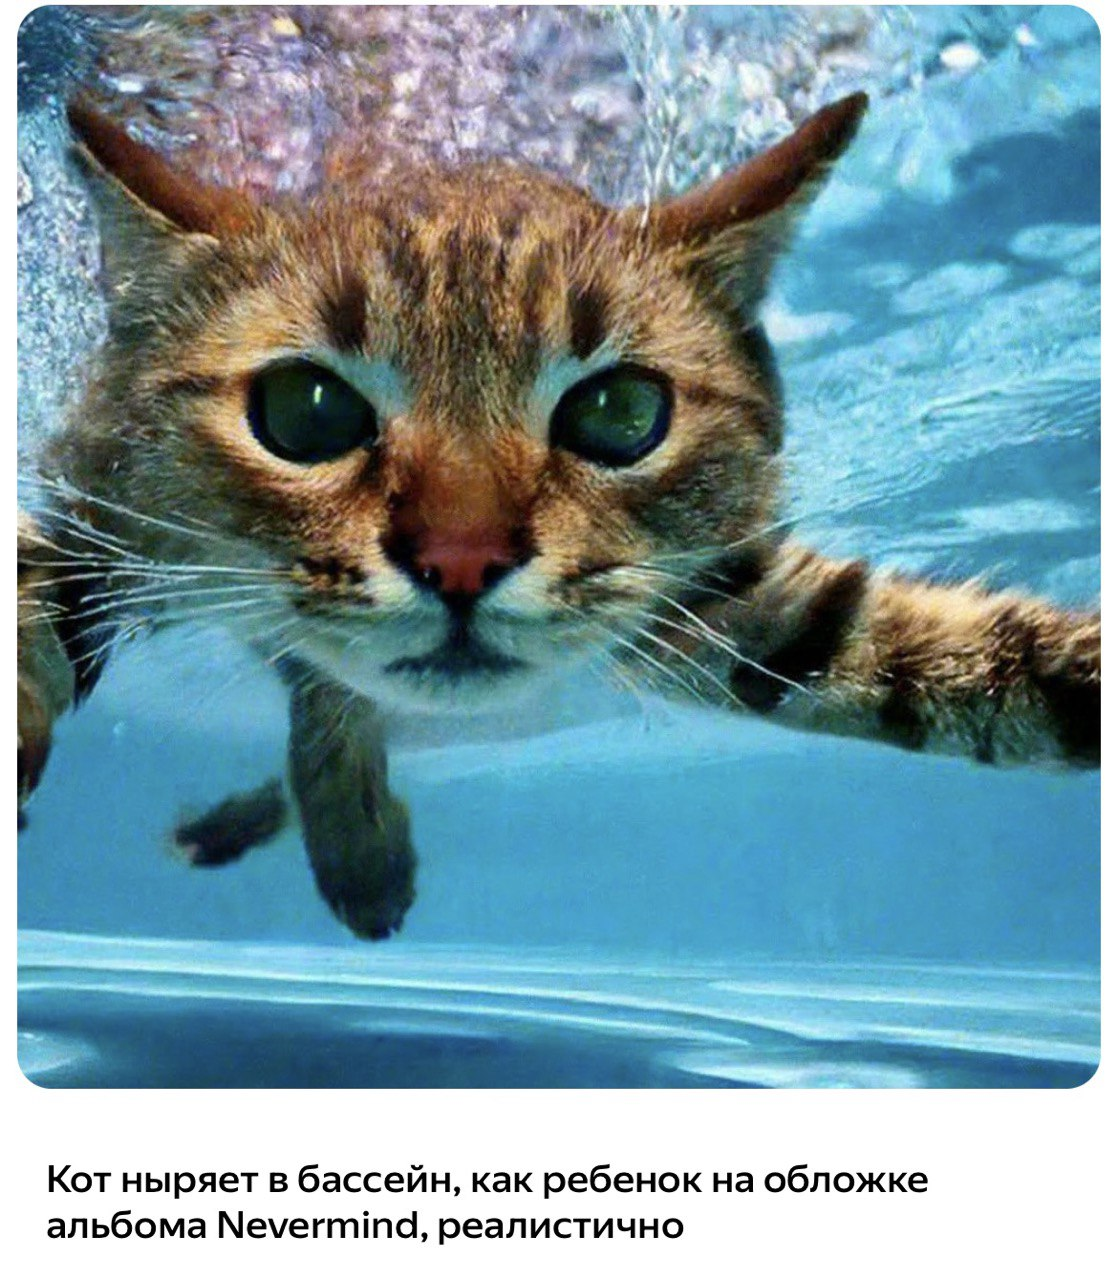
\includegraphics[width=0.9\linewidth]{figs/shedevrum1}
		\end{figure}
	\end{minipage}%
	\begin{minipage}[t]{0.5\columnwidth}
		\begin{figure}
			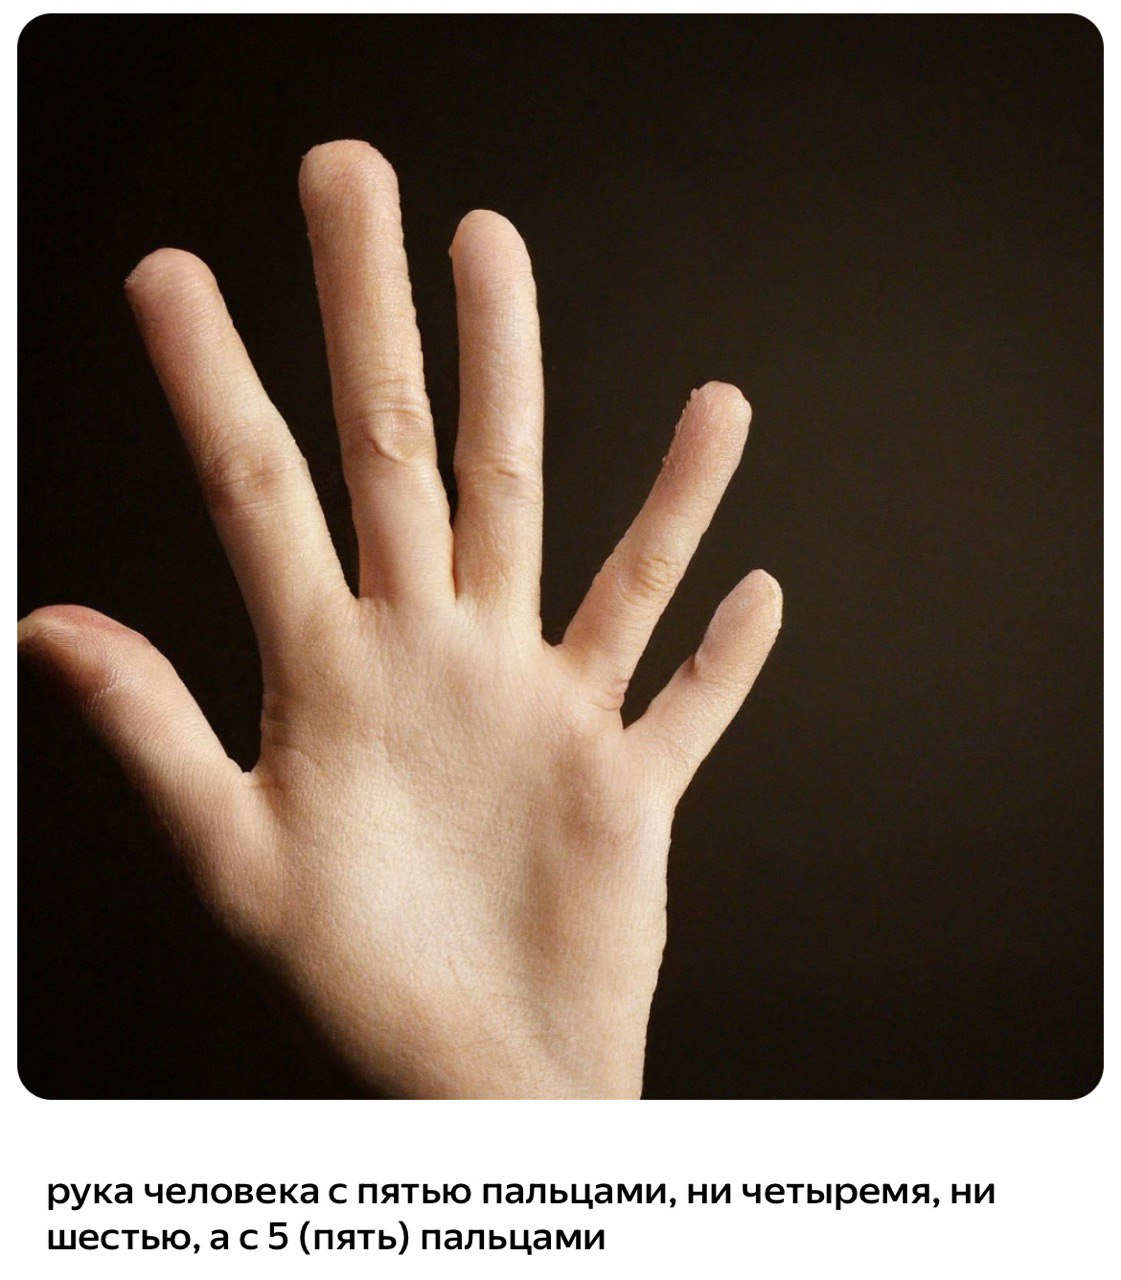
\includegraphics[width=0.9\linewidth]{figs/shedevrum2}
		\end{figure}
	\end{minipage}
\end{frame}
%=======
\begin{frame}{Conditional Models}
	In practice, we're typically interested in learning conditional models (sampling from conditional distribution~$\pd(\bx | \by)$). 
	\begin{itemize}
		\item $\by = \emptyset$, $\bx$ = image $\quad\Rightarrow\quad$ unconditional image model
		\item $\by$ = class label, $\bx$ = image $\quad\Rightarrow\quad$ class-conditional image model
		\item $\by$ = text prompt, $\bx$ = image $\quad\Rightarrow\quad$ text-to-image model
		\item $\by$ = image, $\bx$ = image $\quad\Rightarrow\quad$ image-to-image model
		\item $\by$ = image, $\bx$ = text $\quad\Rightarrow\quad$ image-to-text (image captioning) model
		\item $\by$ = English text, $\bx$ = Russian text $\quad\Rightarrow\quad$ sequence-to-sequence model (machine translation) model
		\item $\by$ = sound, $\bx$ = text $\quad\Rightarrow\quad$ speech-to-text (automatic speech recognition) model
		\item $\by$ = text, $\bx$ = sound $\quad\Rightarrow\quad$ text-to-speech model
	\end{itemize}
\end{frame}
%=======
\begin{frame}{Label Guidance}
	\myfootnotewithlink{https://arxiv.org/abs/1906.00446}{Razavi A., Oord A., et al. Generating Diverse High-Fidelity Images with VQ-VAE-2, 2019}
	\textbf{Label:} Ostrich (10th ImageNet class) 
	\begin{figure}
		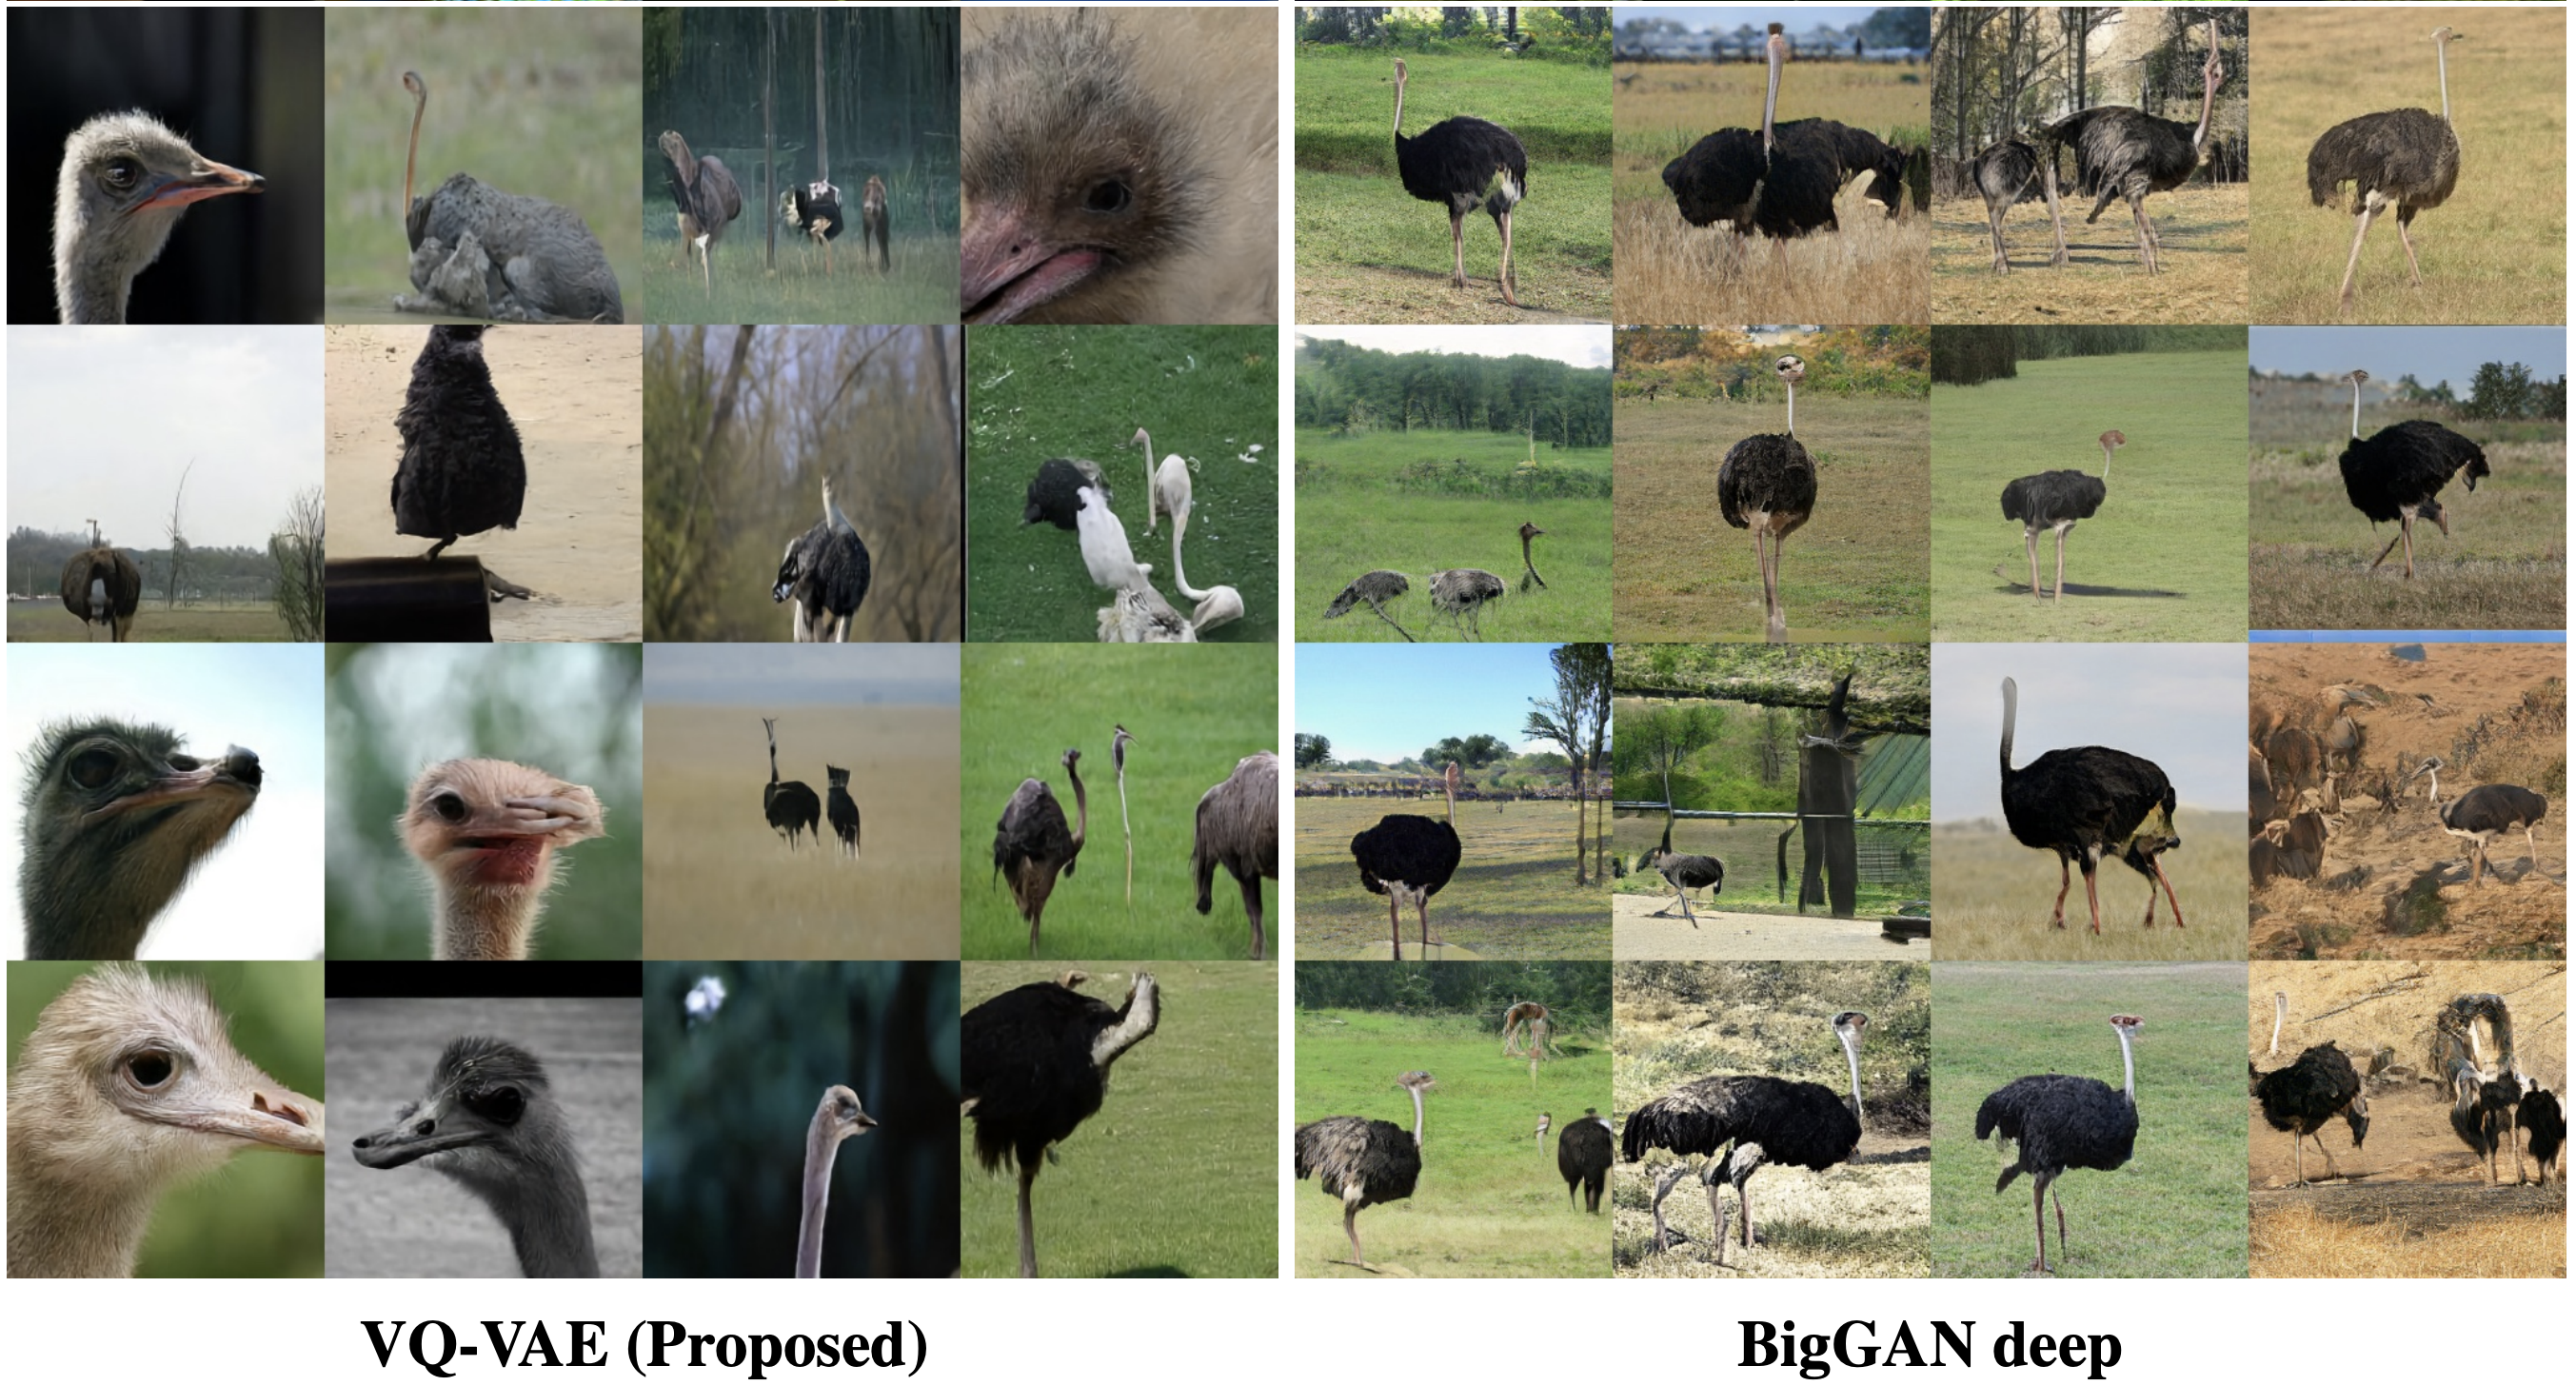
\includegraphics[width=\linewidth]{figs/label_conditioning}
	\end{figure}
\end{frame}
%=======
\begin{frame}{Text Guidance}
	\myfootnotewithlink{https://arxiv.org/abs/2112.10741}{Nichol A., et al. GLIDE: Towards Photorealistic Image Generation and Editing with Text-Guided Diffusion Models, 2022}
	\textbf{Prompt:} a stained glass window of a panda eating bamboo \\
	Left: $\gamma = 1$, Right: $\gamma = 3$.
	\begin{figure}
		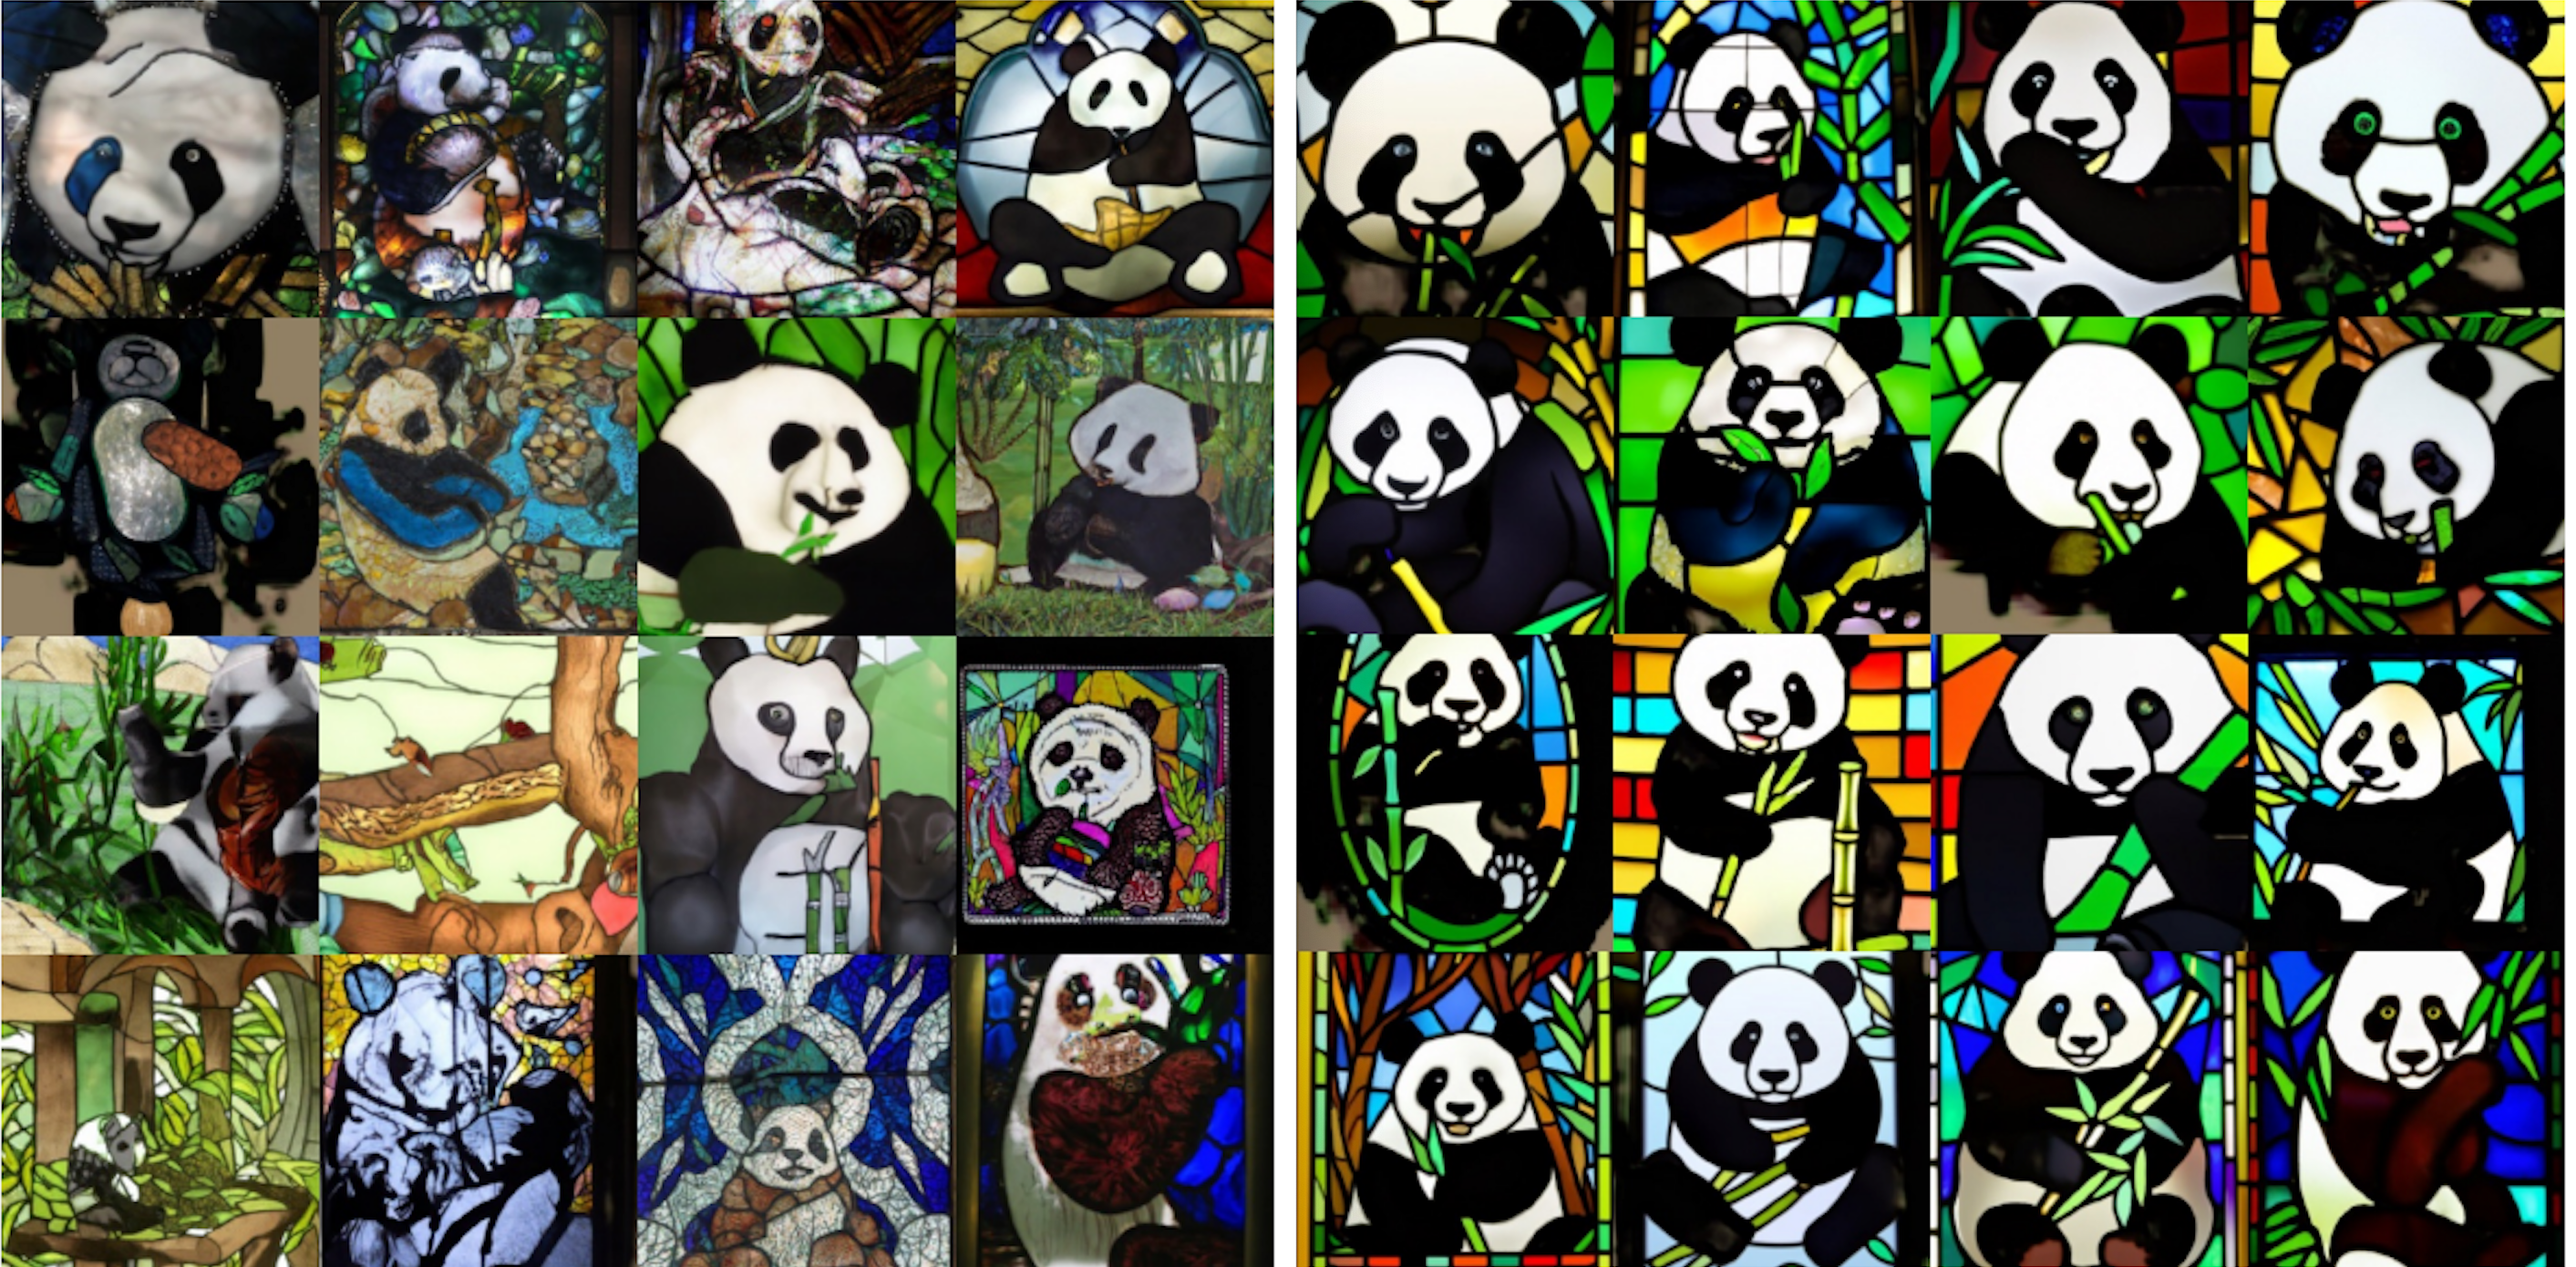
\includegraphics[width=\linewidth]{figs/cfg}
	\end{figure}
\end{frame}
%=======
\begin{frame}{Guidance in Generative Models}
	\begin{block}{How to make guided model?}
		Instead of sampling from $\pt(\bx)$, we sample from $\pt(\bx | \by)$.
	\end{block}
	\eqpause
	Given \textbf{supervised} data $\{(\bx_i, \by_i)\}_{i=1}^n$, we can treat $\by$ as an additional model input:
	\eqpause
	\begin{itemize}
		\item $\pt(x_j | \bx_{1:j-1}, {\color{olive}\by})$ for AR models;
		\eqpause
		\item Encoder $q_{\bphi}(\bz | \bx, {\color{olive}\by})$ and decoder $\pt(\bx | \bz, {\color{olive}\by})$ for VAEs;
		\eqpause
		\item $G_{\btheta}(\bz, {\color{olive}\by})$ for NFs and GANs;
		\eqpause
		\item $\pt(\bx_{t-1} | \bx_t, {\color{olive}\by})$ for DDPMs.
	\end{itemize}
	\eqpause
	\begin{block}{Challenge}
		\begin{itemize}
			\item Empirically, images sampled with this procedure do not fit well enough to the desired label $\by$.
			\item Being able to control the strength of guidance is especially valuable.
		\end{itemize}
	\end{block}
\end{frame}
%=======

\subsection{Classifier Guidance}
%=======
\begin{frame}{Classifier Guidance}
	\myfootnotewithlink{https://arxiv.org/abs/2105.05233}{Dhariwal P., Nichol A. Diffusion Models Beat GANs on Image Synthesis, 2021}
	\begin{block}{DDPM Sampling}
		\begin{enumerate}
			\item Sample $\bx_T \sim \cN(0, \bI)$.
			\item Generate the denoised image (unconditional generation):
			\vspace{-0.3cm}
			\begin{align*}
				\bx_{t - 1} &= \frac{1}{\sqrt{1 - \beta_t}} \cdot \bx_t + \frac{\beta_t}{\sqrt{1 - \beta_t}} \cdot {\color{teal}\bs_{\btheta, t} (\bx_t)} +  \sigma_t \cdot \bepsilon \\
				\nextonslide{
				& = \frac{1}{\sqrt{1 - \beta_t}} \cdot \bx_t + \frac{\beta_t}{\sqrt{1 - \beta_t}} \cdot {\color{teal} \nabla_{\bx_t} \log \pt(\bx_t)} +  \sigma_t \cdot \bepsilon
				}
			\end{align*}
			\vspace{-0.5cm}
		\end{enumerate}
	\end{block}
	\eqpause
	\begin{block}{Guided Generation}
		\vspace{-0.5cm}
		\[
			\bx_{t - 1} = \frac{1}{\sqrt{1 - \beta_t}}\cdot \bx_t +  \frac{\beta_t}{\sqrt{1 - \beta_t}}  \cdot  \nabla_{\bx_t} \log \pt(\bx_t | {\color{olive}\by}) +  \sigma_t \cdot \bepsilon
		\]
		\vspace{-0.3cm}
	\end{block}
	\eqpause
	What is the link between $\nabla_{\bx_t} \log \pt(\bx_t)$ and $\nabla_{\bx_t} \log \pt(\bx_t | {\color{olive}\by})$?
\end{frame}
%=======
\begin{frame}{Classifier Guidance: Guided Score Function}
	\myfootnotewithlink{https://arxiv.org/abs/2105.05233}{Dhariwal P., Nichol A. Diffusion Models Beat GANs on Image Synthesis, 2021}
	\begin{block}{Guided Generation}
		\vspace{-0.5cm}
		\[
			\bx_{t - 1} = \frac{1}{\sqrt{1 - \beta_t}}\cdot \bx_t +  \frac{\beta_t}{\sqrt{1 - \beta_t}}  \cdot {\color{olive} \nabla_{\bx_t} \log \pt(\bx_t | \by)} +  \sigma_t \cdot \bepsilon
		\]
		\vspace{-0.5cm}
	\end{block}
	\eqpause
	\begin{block}{Guided Generation}
		\vspace{-0.7cm}
		\begin{align*}
			{\color{olive}\nabla_{\bx_t} \log \pt(\bx_t | \by)} &= \nabla_{\bx_t} \log \left(\frac{\pt(\bx_t)p(\by | \bx_t)}{p(\by)} \right)\\
			\nextonslide{
			&= {\color{violet}\nabla_{\bx_t} \log \pt(\bx_t)} + \nabla_{\bx_t} \log p(\by | \bx_t) \\
			}
			\nextonslide{
			&= {\color{violet} \bs_{\btheta, t}(\bx_t)} + {\color{teal}\nabla_{\bx_t} \log p(\by | \bx_t)}
			}
		\end{align*}
	\end{block}
	\vspace{-0.5cm}
	\eqpause
	\begin{block}{Guided Score Function}
		\vspace{-0.3cm}
		\[
			\bs_{\btheta, t}(\bx_t, \by) = \nabla_{\bx_t} \log \pt(\bx_t | \by).
		\]
		\eqpause
		\vspace{-0.3cm}
		\[
			{\color{olive}\bs_{\btheta, t}(\bx_t, \by)} = {\color{violet}\bs_{\btheta, t}(\bx_t)} + {\color{teal}\nabla_{\bx_t} \log p(\by | \bx_t)}
		\]
	\end{block}
\end{frame}
%=======
\begin{frame}{Classifier Guidance: Guidance Scale}
	\myfootnotewithlink{https://arxiv.org/abs/2105.05233}{Dhariwal P., Nichol A. Diffusion Models Beat GANs on Image Synthesis, 2021}
	\begin{block}{Guided Score Function}
		\vspace{-0.3cm}
		\[
			{\color{olive}\bs_{\btheta, t}(\bx_t, \by)} = \bs_{\btheta, t}(\bx_t) + \nabla_{\bx_t} \log p(\by | \bx_t)
		\]
		\vspace{-0.5cm}
	\end{block}
	\eqpause
	\begin{itemize}
		\item Let us assume $\by$ is a class label.
		\item $p(\by | \bx_t)$ is a classifier for noisy inputs.
		\item $p(\by | \bx_t)$ is responsible for model guidance.
	\end{itemize}
	\eqpause
	\begin{block}{Guidance Scale}
		It is a natural idea to scale up the contribution of the guidance
		\[
			{\color{violet}\bs^{\gamma}_{\btheta, t}(\bx_t, \by)} = \bs_{\btheta, t}(\bx_t) + {\color{teal}\gamma} \cdot \nabla_{\bx_t} \log p(\by | \bx_t)
		\]
		\eqpause
		\vspace{-0.5cm}
		\begin{itemize}
			\item The {\color{teal}guidance scale $\gamma$} adjusts the strength of classifier guidance.
			\item ${\color{violet}\bs^{\gamma}_{\btheta, t}(\bx_t, \by)}$ is not the true guided score function ${\color{olive}\bs_{\btheta, t}(\bx_t, \by)}$.
		\end{itemize}
	\end{block}
\end{frame}
%=======
\begin{frame}{Classifier Guidance: Distribution Sharpening}
	\myfootnotewithlink{https://arxiv.org/abs/2105.05233}{Dhariwal P., Nichol A. Diffusion Models Beat GANs on Image Synthesis, 2021}
	\begin{block}{Scaled Guided Score Function}
		\[
			{\color{violet}\bs^{\gamma}_{\btheta, t}(\bx_t, \by)} = \bs_{\btheta, t}(\bx_t)+ {\color{teal}\gamma} \cdot \nabla_{\bx_t} \log p(\by | \bx_t)
		\]
		\vspace{-0.5cm}
	\end{block}
	\eqpause
	\begin{block}{Scaled Conditional Distribution}
		\vspace{-0.5cm}
		\begin{align*}
			{\color{violet}\nabla_{\bx_t}^{\gamma} \log \pt(\bx_t | \by)} 
			&= \nabla_{\bx_t} \log \pt(\bx_t) + {\color{teal}\gamma}  \cdot \nabla_{\bx_t} \log p(\by | \bx_t) \\
			\nextonslide{
			&= \nabla_{\bx_t} \log \pt(\bx_t) + \nabla_{\bx_t} \log p(\by | \bx_t)^{\color{teal}\gamma} \\
			}
			\nextonslide{
			&= \nabla_{\bx_t} \log \left( \frac{\pt(\bx_t) p(\by | \bx_t)^{\gamma}}{Z} \right)
			}
		\end{align*}
		\vspace{-0.3cm}
	\end{block}
	\eqpause
	\textbf{Note:} Increasing $\gamma$ sharpens $p(\by | \bx_t)$, making it more contrast
	\[
		\hat{p}(\by | \bx_t) \propto p(\by | \bx_t)^{\gamma}.
	\]
\end{frame}
%=======
\begin{frame}{Classifier Guidance: Overview}
	\myfootnotewithlink{https://arxiv.org/abs/2105.05233}{Dhariwal P., Nichol A. Diffusion Models Beat GANs on Image Synthesis, 2021}

	\begin{block}{Training}
		\begin{itemize}
			\item Train the DDPM as before.
			\item Train an additional classifier $p(\by | \bx_t)$ on noisy data (note that it is dependent on time $t$).
		\end{itemize}
		\vspace{-0.2cm}
	\end{block}
	\eqpause
	\begin{block}{Guided DDPM Sampling}
		\begin{enumerate}
			\item Sample $\bx_T \sim \cN(0, \bI)$.
			\item Generate the denoised image (using scaled guided score function):
			\[
				\bx_{t-1} = \frac{1}{\sqrt{1 - \beta_t}} \cdot \bx_t + \frac{\beta_t}{\sqrt{1 - \beta_t}} \cdot  {\color{olive}\bs^{\gamma}_{\btheta, t}(\bx_t, \by)} + \sigma_t \cdot \bepsilon
			\]
		\end{enumerate}
	\end{block}
\end{frame}
%=======
\subsection{Classifier-Free Guidance}
%=======
\begin{frame}{Classifier-Free Guidance}
	\myfootnotewithlink{https://arxiv.org/abs/2207.12598}{Ho J., Salimans T. Classifier-Free Diffusion Guidance, 2022}
	\begin{itemize}
		\item The previous approach relies on training an additional classifier $p(\by | \bx_t)$ for noisy images.	
		\item We now introduce a method to sidestep this requirement.
	\end{itemize}
	\eqpause
	\[
		\nabla_{\bx_t}^{\gamma} \log \pt(\bx_t | \by) = \nabla_{\bx_t} \log \pt(\bx_t) + \gamma \cdot {\color{teal}\nabla_{\bx_t} \log p(\by | \bx_t)}
	\]
	\eqpause
	\vspace{-0.5cm}
	\begin{block}{Bayes theorem}
		\vspace{-0.7cm}
		\begin{align*}
			{\color{teal}\nabla_{\bx_t} \log p(\by | \bx_t)} &= \nabla_{\bx_t} \log \left( \frac{\pt(\bx_t| \by) p(\by)}{\pt(\bx_t)} \right) \\
			\nextonslide{
			&=  \nabla_{\bx_t} \log \pt(\bx_t| \by) -\nabla_{\bx_t} \log  \pt(\bx_t)
			}
		\end{align*}
	\end{block}
	\eqpause
	\vspace{-0.5cm}
	\begin{block}{Scaled Guided Score Function}
		\vspace{-0.7cm}
		\begin{multline*}
			\nabla_{\bx_t}^{\gamma} \log \pt(\bx_t | \by) = \nabla_{\bx_t} \log \pt(\bx_t) + \gamma \cdot {\color{teal} \nabla_{\bx_t} \log p(\by | \bx_t)}
			\nextonslide{ = \\ = \nabla_{\bx_t} \log \pt(\bx_t) + \gamma \cdot \bigl( {\color{teal}\nabla_{\bx_t} \log \pt(\bx_t| \by) - \nabla_{\bx_t} \log  \pt(\bx_t)} \bigr)}
			\nextonslide{ = \\ =  (1 - \gamma) \cdot  \nabla_{\bx_t} \log \pt(\bx_t) + \gamma \cdot  \nabla_{\bx_t} \log \pt(\bx_t| \by)}
		\end{multline*}
	\end{block}
\end{frame}
%=======
\begin{frame}{Classifier-Free Guidance: Formulation}
	\myfootnotewithlink{https://arxiv.org/abs/2207.12598}{Ho J., Salimans T. Classifier-Free Diffusion Guidance, 2022}
	\begin{block}{Scaled Guided Score Function}
		\vspace{-0.5cm}
		\[
			\nabla_{\bx_t}^{\gamma} \log \pt(\bx_t | \by) =  (1 - \gamma) \cdot  \nabla_{\bx_t} \log \pt(\bx_t) + \gamma \cdot  \nabla_{\bx_t} \log \pt(\bx_t| \by)
		\]
		\vspace{-0.5cm}
		\eqpause
		\[
			\bs^{\gamma}_{\btheta, t}(\bx_t, \by) = (1 - \gamma) \cdot \bs_{\btheta, t}(\bx_t) +  \gamma \cdot \bs_{\btheta, t}(\bx_t, \by)
		\]
		\vspace{-0.5cm}
	\end{block}
	\eqpause
	\begin{block}{Naive training approach}
		\begin{itemize}
			\item Train an unguided score function model $\bs_{\btheta, t}(\bx_t)$.
			\item Train a guided score function model $\bs_{\btheta, t}(\bx_t, \by)$.
			\eqpause
			\item Use their convex combination at inference.
		\end{itemize}
	\end{block}
	\begin{block}{Guided Sampling}
		\vspace{-0.3cm}
		\[
			\bx_{t-1} = \frac{1}{\sqrt{1 - \beta_t}} \cdot \bx_t + \frac{\beta_t}{\sqrt{1 - \beta_t}} \cdot  {\color{olive}\bs^{\gamma}_{\btheta, t}(\bx_t, \by)} + \sigma_t \cdot \bepsilon
		\]
		\vspace{-0.3cm}
	\end{block}
	\eqpause
	How to avoid training two separate score function models?
\end{frame}
%=======
\begin{frame}{Classifier-Free Guidance}
	\myfootnotewithlink{https://arxiv.org/abs/2506.02070}{Holderrieth P., Erives E. An Introduction to Flow Matching and Diffusion Models, 2025}
	\[
		\bs^{\gamma}_{\btheta, t}(\bx_t, \by) = (1 - \gamma) \cdot \bs_{\btheta, t}(\bx_t) +  \gamma \cdot \bs_{\btheta, t}(\bx_t, \by)
	\]
	\vspace{-0.5cm}
	\begin{block}{CFG algorithm}
		\begin{itemize}
			\item Introduce "the absence of conditioning" label $\by = \varnothing$.		
			\eqpause
			\item Use it to get unguided score function $\bs_{\btheta, t}(\bx_t) = \bs_{\btheta, t}(\bx_t, \varnothing)$.		
			\eqpause
			\item Train a single model $\bs_{\btheta, t}(\bx_t, \by)$ using \textbf{supervised} data, but artificially drop the labels $\by$ with some fixed probability (simulating the case of $\by = \varnothing$).		
			\eqpause
			\item Apply the model twice during inference to get $\bs_{\btheta, t}(\bx_t, \varnothing)$ and $\bs_{\btheta, t}(\bx_t, \by)$.
		\end{itemize}
	\end{block}
	\vspace{-0.3cm}
	\eqpause
	\begin{block}{Guided Sampling}
		\vspace{-0.3cm}
		\[
			\bx_{t-1} = \frac{1}{\sqrt{1 - \beta_t}} \cdot \bx_t + \frac{\beta_t}{\sqrt{1 - \beta_t}} \cdot  {\color{olive}\bs^{\gamma}_{\btheta, t}(\bx_t, \by)} + \sigma_t \cdot \bepsilon
		\]
		\vspace{-0.3cm}
	\end{block}
\end{frame}
%=======
\begin{frame}{Summary}
    \begin{itemize}
        \item At each step, DDPM predicts the noise that was injected in the forward process. 
        \vfill
        \item DDPMs are quite slow, since the model must be applied $T$ times for sampling.	
		\vfill
		\item DDPM and NCSN are intimately connected at the objective level.
		\vfill
		\item Guidance technique allows to make controllable generation via conditioning on labels or text prompts.
        \vfill 
		\item Classifier guidance turns an unconditional model into a conditional one by training an auxiliary classifier on noisy data.
		\vfill
		\item Classifier-free guidance removes the need for such a classifier, yielding a practical recipe now widely used.
    \end{itemize}
\end{frame}
%=======
\end{document}